\chapter{Benchmarks en Experimenten}
% \chaptermark{Een kortere titel voor de paginahoofding (verschillend van titel in TOC)}

In dit hoofdstuk bespreken we alle uitgevoerde experimenten, zowel op kleine- als grote schaal, om de schaalbaarheid van de \nwmretriever{} te onderzoeken.

Op kleine schaal maken we gebruik van virtuele machines en een aantal productieswitches om onze testen uit te voeren.
We onderzoeken de impact van netwerkvertraging, het nut van het filteren van de gegevens die moeten opgehaald worden, en de impact van bulkrequests.
Verder vergelijken we de performantie van de \nwmretriever{} met de Net-SNMP commandlinetools,
analyseren we de \nwmretriever{} nader met een profiler, onderzoeken we of het beter is om een tabel rij per rij of kolom per kolom op te vragen,
en gaan we na wat de impact is van de fragmentatie van pakketten op het netwerk.

Bij het identificeren van problemen die de schaalbaarheid belemmeren, bespreken en implementeren we oplossingen.
Achteraf analyseren we ook de effectiviteit van die oplossingen.

Dankzij de samenwerking met het iMinds onderzoekscentrum kunnen we op grote schaal gebruik maken van de Virtual Wall die toelaat om snel geautomatiseerde testnetwerken op te zetten.
We maken gebruik van virtualisatie om een groot aantal toestellen te creëren die we kunnen bevragen via SNMP.
Met dat groot aantal toestellen kunnen we de uitvoeringstijd, het CPU-, geheugen- en bandbreedtegebruik analyseren die op grote schaal nodig is.
We kijken hierbij naar zowel de originele versie van de \nwmretriever{}, als de versie met onze verbeteringen,
om te zien of ze het gewenste effect hebben op de schaalbaarheid.


\section{Terminologie}

Alvorens we beginnen met de benchmarks en experimenten, willen we nog eens de gebruikte terminologie verduidelijken, zodat er zeker geen verwarring ontstaat.

Om te beginnen worden gegevens die een \gls{snmp-agent} aanbiedt, voorgesteld door \textbf{objecten}.
Een object wordt uniek geïdentificeerd door een \textbf{\gls{oid}}.
Omdat \glspl{oid} hiërarchisch zijn opgebouwd, komt een \gls{oid} niet noodzakelijk overeen met juist één object.
Als we een hoger gelegen \gls{oid} opvragen, krijgen we dus meerdere gegevens terug.

Typisch overlopen we een hoger gelegen \gls{oid} met een SNMP walkopdracht.
Deze blijft gegevens lexicografisch overlopen totdat de opgehaalde gegevens niet meer onder de originele \gls{oid} vallen.
Alle gegevens die wel onder de originele \gls{oid} vallen, noemen we \textbf{relevant}.
Maar omdat je extra gegevens moet opvragen om te weten dat er geen gegevens meer onder de originele \gls{oid} vallen,
hebben we ook een aantal \textbf{niet-relevante gegevens}.

Ten slotte zijn er twee retrievers waarvan we gebruik maken om SNMP-gegevens op te halen.
Enerzijds hebben we de \textbf{\nwmretriever{}} van NetworkMining en anderzijds zijn er de Net-SNMP commandlinetools.

\section{Kleinschalige benchmarks en experimenten}

\todo[inline]{Geen inleiding nodig?}

\subsection{Virtuele machines}
\label{virtualbox}

\todo[inline]{Betere titel! Virtuele testopstelling van een handvol switches.}

\todo[inline, caption={}]{
Bespreking originele testopstelling van Wouter Tavernier? \\
Specs \\
Software(config)

\begin{itemize}
	\item screen (niet geinstalleerd)
	\item sudo
	\item snmpd
	\item snmp
	\item snmp-mibs-downloader
	\item bridge, lldp...
\end{itemize}


}

De eerste testopstelling bestaat uit vier virtuele machines die switches in een netwerk nabootsen.
Als virtualisatieplatform wordt er gebruik gemaakt van \textit{Oracle VM VirtualBox} (verder gewoon VirtualBox genoemd).
VirtualBox is vrij te verkrijgen voor alle gangbare besturingssystemen en is bovendien open-source.

\subsubsection{Hardwareconfiguratie}

Aan elke node wordt 256 MB geheugen en één CPU-\textit{core} toegewezen.
Op de nodes wordt een minimale versie van Debian 7 geïnstalleerd, zonder grafische schil.
Hierdoor is zelfs 256 MB een ruime luxe voor de nodes: na het opstarten van een node wordt er amper 70MB geheugen gebruikt.

Alle toestellen zijn rechtstreeks met elkaar verbonden in een privénetwerk.
Via \gls{nat} kunnen ze via de gastheer toch nog het internet bereiken.
Dit werd bewerkstelligd met de \textit{NAT Network mode},
een nieuwe feature in VirtualBox die nog niet in de documentatie staat, maar wel kort beschreven wordt in een nieuwspost (zie\cite{vbox-nat-network-mode}).
Ter vergelijking:
\textit{NAT mode} laat gastsystemen toe om met het internet te communiceren via \gls{nat}, maar zitten elk in een apart privénetwerk en kunnen dus niet met elkaar praten.
\textit{Host-only mode} laat gastsystemen met elkaar (en het gastheersysteem) communiceren door ze in een gezamelijk privénetwerk te plaatsen, 
maar communicatie met het internet is niet mogelijk.

\subsubsection{Softwareconfiguratie}

Hieronder leggen we kort stap voor stap uit hoe je op een Debianinstallatie de nodige SNMP software kunt installeren en configureren.
De uitleg is zeer beknopt gehouden en dient enkel om je op weg te helpen.
In de testopstelling werden de nodes ook nog geconfigureerd als switches die het \gls{stp} uitvoeren, alsook het \gls{lldp}.
Deze extra protocollen bieden informatie aan die via SNMP opgevraagd kan worden en dit zijn ook gegevens die in een realistische situatie opgevraagd kunnen worden.
De configuratie als switch en van LLDP wordt hier echter niet besproken. \todo{Dit kan eventueel als bijlage uitgelegd worden.}

Om de nodes van een minimale Debian 7 installatie te voorzien, werden geen extra softwarepakketten geselecteerd bij de installatie.

In de veronderstelling dat het internet werkt, beginnen we na de installatie met het updaten van het systeem en het installeren van \textit{sudo}:

\begin{lstlisting}[language=bash]
# apt-get update
# apt-get upgrade
# apt-get install sudo
\end{lstlisting}

Maak een gebruiker aan en zorg ervoor dat je sudo rechten hebt met behulp van het \textit{visudo} commando of door je gebruiker toe te voegen aan de \textit{sudo} groep.

\begin{lstlisting}[language=bash]
# visudo
# usermod -a -G sudo <jouw gebruikersnaam>
\end{lstlisting}

Dan installeren we de snmp \textit{daemon} die zal antwoorden op SNMP requests.
Om te testen is het ook interessant om de client-side SNMP tools te installeren, alsook een tool om de belangrijkste \glspl{mib} te downloaden.
Met die \glspl{mib} kunnen numerieke \glspl{oid} omgezet worden naar de meer gebruiksvriendelijke tekstuele voorstelling.

Debian laat standaard niet toe dat niet-vrije (non-free) software\footnote{
	Dit is software die niet volledig vrij is maar op een of andere manier beperkt wordt door zijn licentie. De eisen die gesteld worden aan vrije software voor Debian zijn te vinden in de Debian Free Software Guidelines (DFSG)\cite{dfsg}\cite{dfsg-wiki}.}
geïnstalleerd wordt. De \textit{snmp-mibs-downloader} tool die we nodig hebben om de \glspl{mib} te downloaden is daar een voorbeeld van.
Om dit toch toe te laten moet je voor elke lijn in /etc/apt/sources.list het non-free-component achteraan toevoegen.
Dan krijg je zoiets:

\begin{lstlisting}[language=bash]
deb http://ftp.belnet.be/debian wheezy main non-free
deb-src http://ftp.belnet.be/debian wheezy main non-free
\end{lstlisting}

Nu kunnen we wel snmp-mibs-downloader en de andere tools installeren.

\begin{lstlisting}[language=bash]
$ sudo apt-get install snmpd snmp snmp-mibs-downloader
\end{lstlisting}

Het volgende commando zal de \glspl{mib} downloaden:

\begin{lstlisting}[language=bash]
$ sudo download-mibs
\end{lstlisting}

Het gebruik van de \glspl{mib} kun je aanzetten door de volgende regel in commentaar te zetten in het bestand /etc/snmp/snmp.conf:

\begin{lstlisting}[language=bash]
mibs :
\end{lstlisting}

Om \textit{snmpd} te configureren, kun je gebruik maken van het \textit{snmpconf} commando, dat op interactieve wijze configuratiebestanden aanmaakt.
We moeten ook nog de locatie van de \gls{mib}-bestanden opgeven. Voeg daarom het volgende toe aan /etc/default/snmpd:

\begin{lstlisting}[language=bash]
export MIBS=/usr/share/mibs
\end{lstlisting}

Vervolgens herstarten we snmpd om de nieuwe configuratie in te laden.

\begin{lstlisting}[language=bash]
$ sudo /etc/init.d/snmpd restart
\end{lstlisting}

Om te testen of alles werkt, gebruiken we het volgende commando:

\begin{lstlisting}[language=bash]
$ snmpwalk -v 1 -c public localhost mib-2
\end{lstlisting}

\todo[inline]{Verder eventueel: bridge configuratie, LLDP}

\todo[inline]{SNMP Data Retriever in een Windows XP VM?}


\subsection{Productieswitches}

\todo[inline]{Betere titel? Fysieke "testopstelling" van een handvol switches. Niet echt een testopstelling natuurlijk, maar wel echte productieswitches.}

Naast een viertal virtuele machines kunnen we ook gebruik maken van tien productieswitches die deel uitmaken van het netwerk van iMinds.
Deze switches kunnen we gebruiken om na te gaan of de tests met de virtuele machines de realiteit goed kunnen benaderen.
Er worden drie verschillende modellen gebruikt van verschillende grootte en functionaliteit.
De grootste bevat bijna 300 poorten en functioneert ook als router.

\subsection{Netwerkvertraging}
\label{latency}

Netwerkvertraging of \textit{latency} definiëren we als de zogenaamde \textit{round-trip time},
of de totale tijd die nodig is om een bericht te sturen naar een ander toestel en voor die computer om het antwoord terug naar jou te sturen\footnote{
	Latency kan ook gedefiniëerd worden als enkel de tijd dat een bericht nodig heeft om in één richting reizen.
	Dat is echter moeilijker om te meten. Meestal hanteert men de round-trip time omdat dat gemeten kan worden vanaf slechts een punt. \cite{latency-wiki}
}.
De latency tussen twee toestellen kan je gemakkelijk meten vanop een van de twee toestellen met behulp van het \textit{ping}-commando.

Op een LAN-netwerk bedraagt de latency gewoonlijk minder dan 1 ms en valt dus te verwaarlozen.
Zodra netwerkverkeer over het internet moet gaan, speelt latency wel een grote rol.
Zolang de afstand niet te groot is (als we binnen West-Europa blijven), blijft de latency beperkt tot 10-50 ms.
Als we daarentegen communiceren met bv. Amerika, dan spreken we al over 100-200 ms (respectievelijk voor de Oost- en Westkust).
Voor sommige toepassingen (zoals bijvoorbeeld real-time spellen) is dit te hoog om nog bruikbaar te zijn.

Het belang voor ons van de latency is voornamelijk bij het opvragen van veel gegevens met GET- en GETNEXT-requests.
Zoals uitgelegd in \cref{snmp-operaties}, wordt er slechts één gegeven in een request gestopt en
moet je steeds wachten op het antwoord ervan, alvorens je de volgende request stuurt.
Als je te maken hebt met een latency van zeg maar 25 ms, dan wil dat zeggen dat je steeds 25 ms moet wachten alvorens je de volgende request kunt sturen.
Stel dat je 200 gegevens wenst op te halen, dan doe je hier 5 seconden over (200 gegevens $*$ 25 ms wachten per gegeven).

Was er een netwerkvertraging van slechts 1 ms, dan zou het ophalen van dezelfde 200 gegevens nog maar 200 ms duren.
Natuurlijk houden we hier nog geen rekening met de tijd die het toestel zelf nodig heeft om het bericht te verwerken en te beantwoorden.

De originele versie van de SNMP Data Retriever maakte gebruik van GET- en GETNEXT-requests en ondervond dus een grote invloed op de uitvoeringstijd door de netwerkvertraging.
Om na te gaan hoe groot de impact juist is, hebben we tests gedaan met en zonder netwerkvertraging.

\subsubsection{Meetresultaten}

Deze tests hebben we gedaan op de virtuele machines omdat je in Linux gemakkelijk een artificiële netwerkvertraging kunt creëren.
Daarvoor gebruik je het volgende commando:

\begin{lstlisting}[language=bash, caption={Artificiële netwerkvertraging creëren in Linux}]
$ sudo tc qdisc add dev eth0 root netem delay 25 ms
\end{lstlisting}

Dit commando zorgt ervoor dat er een latency van 25 ms gecreëerd wordt op de \textit{eth0} interface.
\todo[]{Is een vertraging van 25 ms wel realistisch?}
We hebben de test gedaan met de originele versie van de SNMP Data Retriever bij het ondervragen van een of meerdere machines,
met en zonder netwerkvertraging.

De resultaten zie je in \cref{tabel-latency}.
De eerste rij toont de gemiddelde uitvoeringstijd en de tweede het CPU-gebruik van het (volledige) systeem.

\begin{table}[h]
\centering
\begin{tabular}{@{}lllll@{}}
\toprule
                      & \multicolumn{2}{c}{25 ms vertraging} & \multicolumn{2}{c}{geen vertraging} \\
                      & 1 toestel       & 4 toestellen       & 1 toestel       & 4 toestellen      \\ \midrule
Uitvoeringstijd (s):  & 15,650          & 15,987             & 2,693           & 6,105             \\
CPU-gebruik:          & 10\%            & 35\%               & 80-90\%         & 100\%    		   \\ \bottomrule
\end{tabular}
\caption{De tijd nodig om 1-4 toestellen te ondervragen met en zonder vertraging}
\label{tabel-latency}
\end{table}

Jammer genoeg wordt er per seconde maar één meting van het CPU-gebruik gedaan, waardoor
de kortste test van minder dan drie seconden, bij een toestel zonder vertraging, niet zo nauwkeurig is.
Desondanks is het toch voldoende om te zien dat het CPU-gebruik een bottleneck vormt bij het bevragen van vier toestellen zonder vertraging.
Het moet wel gezegd worden dat de retriever in een virtuele machine draaide waaraan slechts een CPU-core werd toegewezen.\footnote{
	Dit was omdat er een VirtualBox-\textit{image} werd voorzien waarop alles reeds voorgeconfigureerd was om snel te kunnen beginnen met het testen van de retriever.
	Bij latere tests draait de \nwmretriever{} niet meer in een virtuele machine en beschikt ze over meerdere cores.
}.
Ook bij slechts een toestel zonder vertraging zie je dat het CPU-gebruik vrij hoog ligt.
Wanneer we een vertraging van 25 ms introduceren is het CPU-gebruik een stuk lager.
Hadden we 50 toestellen bevraagd --- het maximum aantal dat de retriever tegelijkertijd doet --- met een vertraging van 25 ms,
dan hadden we evenwel weer in de problemen gezeten.

Op het CPU-gebruik komen we later nog terug, maar de belangrijkste reden dat we deze test gedaan hebben, is om de impact op de uitvoeringstijd in te kunnen schatten.
We vragen ongeveer 217 gegevens op per toestel.
Voor één enkel toestel zonder vertraging duurde dit ongeveer 2.700 ms.
Ter vergelijking, volgens onze eerdere rekenformule had dit ongeveer 200 ms moeten duren.
We zaten er dus een factor 10 naast.
Er is natuurlijk flink wat meer aan de hand dan enkel het vervoeren van het pakket over de netwerkverbinding.
De retriever doet namelijk ook een aantal databankinteracties zoals het aanmaken van tabellen en
het wegschrijven van de resultaten in die databank (zie \cref{snmp-data-retriever-db}).

Als we een vertraging van 25 ms invoeren, neemt de uitvoeringstijd toe met bijna een factor 6 tot 15.650 ms.
Onze duidelijk oververeenvoudigde rekensom van daarnet zou uitkomen op een kleine 6 seconden.

Dezelfde vergelijking maken met vier toestellen is jammer genoeg nutteloos vanwege de CPU-bottleneck.
Het is wel interessant om te zien dat het ondervragen van extra toestellen slechts een kleine impact heeft op de uitvoeringstijd.
Logisch, want de vier toestellen worden tegelijkertijd ondervraagd.


\subsubsection{Conclusie}

Het is duidelijk dat de netwerkvertraging een belangrijke rol speelt in de uitvoeringstijd van de retriever.
We raden daarom dan ook sterk aan om, indien mogelijk, de bevragingen \textit{on-site} te doen
(dit wil zeggen op hetzelfde netwerk in plaats van op afstand) om de netwerkvertraging te minimaliseren.

Het effect van de netwerkvertraging kan ook beperkt worden door het gebruik van GETBULK-requests,
waarbij meerdere gegevens in een pakket worden gestopt.
Als je 10 gegevens in een pakket stopt, betekent dat theoretisch al een snelheidwinst van factor 10.
We zullen dit dan ook verder onderzoeken in \cref{bulkrequests-benchmarks}.

\todo[inline]{Dubbelcheck of naar de correcte paragraaf verwezen wordt.
Latency komt wel niet opnieuw aan bod in die paragraaf, beter om de laatste zin hier te herschrijven om te zeggen dat we bulkrequests onderzoeken.}



\subsection{Filteren van de op te vragen gegevens}
\label{fracties}

Een van de vragen die we ons gesteld hebben, is of het wel degelijk de moeite waard is om de gegevens die we opvragen te filteren?
Is het met andere woorden nuttig dat we ons bezighouden met een lijst op te stellen van enkel de \glspl{oid} die ons interesseren,
of kunnen we evengoed meteen alle gegevens opvragen die een \gls{snmp-agent} ons aanbiedt?

\subsubsection{Meetresultaten}

Voor deze test stellen we een lijst op van de typisch meest interessante \glspl{oid} bij netwerkcomponenten.
We bekijken hoeveel objecten die \glspl{oid} ons opleveren en vergelijken dit met het totaal aantal objecten dat een \gls{snmp-agent} aanbiedt.
Omdat de virtuele machines, die als switch geconfigureerd zijn, niet verbonden zijn met echte computers, zullen ze minder gegevens bevatten dan een echte switch.
Anderzijds bevatten de virtuele machines heel wat extra informatie die een gewone switch niet heeft, omdat ze een volledig besturingssysteem draaien.
Denk hierbij aan bijvoorbeeld een lijst van alle geïnstalleerde softwarepakketten.
Omdat het belangrijk is dat deze test de realiteit zo goed mogelijk weergeeft, werd deze test dan ook uitgevoerd op productieswitches.

Dit is de lijst van \glspl{oid} die we als interessant beschouwen:

\begin{lstlisting}
1.3.6.1.2.1.1			(system)
1.3.6.1.2.1.2			(interfaces)
1.3.6.1.2.1.4			(ip)
1.3.6.1.2.1.17.1 		(dot1dBase)
1.3.6.1.2.1.17.2		(dot1dStp)
1.0.8802.1.1.2.1.4.1	(lldpRemTable)
\end{lstlisting}

De twee \glspl{oid} die beginnen met \textit{dot1d} hebben betrekking op de switching functionaliteit.
\textit{dot1dBase} bevat onder andere de tabel met alle switchpoorten terwijl \textit{dot1dStp} informatie bevat over het Spanning Tree Protocol (STP).

Om te bepalen hoeveel objecten er in totaal aangeboden worden, kun je een SNMP walk doen van \gls{oid} '.' of '.1'.

Een voorbeeld van de uitvoer die onze test oplevert is het volgende:

\begin{lstlisting}
Host: atlas1a1.intec.ugent.be
Date: Thu Apr 17 17:20:48 CEST 2014

Retrieved 267 objects for dot1dStp (1.3.6.1.2.1.17.2).
Retrieved 1318 objects for dot1dBase (1.3.6.1.2.1.17.1).
Retrieved 7943 objects for interfaces (1.3.6.1.2.1.2).
Retrieved 7 objects for system (1.3.6.1.2.1.1).
Retrieved 1716 objects for ip (1.3.6.1.2.1.4).
Retrieved 207 objects for lldpRemTable (1.0.8802.1.1.2.1.4.1).
Retrieved 11458 objects in total.
The agent has 369388 objects in total.
Percentage of retrieved objects from total: 3.10188744626247%
\end{lstlisting}

We zien dus hoeveel objecten we terugkrijgen bij het overlopen van elke \gls{oid},
het totaal aantal objecten dat we teruggekregen hebben bij alle voor ons interessante \glspl{oid} en
hoeveel objecten het toestel in totaal aanbiedt (voor alle ondersteunde \glspl{oid}).
Tenslotte zien we ook nog het percentage van interessante objecten t.o.v. het totaal.
Een samenvatting van de resultaten voor de verschillende productieswitches zien we in \cref{tabel-fracties}.
Gemiddeld komen we uit op een percentage van 4,48\% interessante gegevens over alle switches heen.

\begin{table}[h]
\centering
\begin{tabular}{@{}lrrr@{}}
\toprule
Host                    & Interessante objecten & Totaal aantal objecten & Percentage \\ \midrule
atlas1a1.intec.ugent.be & 11.458                & 369.388                & 3,10\%     \\
atlas1a2.intec.ugent.be & 5.636                 & 123.617                & 4,56\%     \\
atlas2a1.intec.ugent.be & 3.247                 & 69.022                 & 4,70\%     \\
atlas2a2.intec.ugent.be & 3.238                 & 69.201                 & 4,68\%     \\
atlas2b1.intec.ugent.be & 3.247                 & 69.418                 & 4,68\%     \\
atlas2b2.intec.ugent.be & 3.238                 & 69.449                 & 4,66\%     \\
atlas3a1.intec.ugent.be & 3.256                 & 69.952                 & 4,65\%     \\
atlas3a2.intec.ugent.be & 3.251                 & 69.509                 & 4,68\%     \\
atlas3b1.intec.ugent.be & 3.247                 & 70.212                 & 4,62\%     \\ \bottomrule
\end{tabular}
\caption{Aantal interessante objecten t.o.v. totaal aantal objecten}
\label{tabel-fracties}
\end{table}

\subsubsection{Conclusie}

Gezien het lage percentage van gegevens die voor ons echt interessant is,
loont het zeker de moeite om een lijst op te stellen van de \glspl{oid} die interessant zijn.
Dit zal sowieso al een groot verschil uitmaken in de uitvoeringstijd omdat er 20 keer minder gegevens moeten opgevraagd worden.
Bovendien moeten er dan ook een pak minder gegevens opgeslagen worden,
zeker als er meerdere kopieën van dezelfde gegevens bijgehouden worden over een bepaalde tijdspanne.


\subsection{Bulkrequests}
\label{bulkrequests-benchmarks}

In \cref{snmp-operaties,latency} bespraken we dat het samenbundelen van meerdere objecten in een request, althans theoretisch, een zeer goed idee is.
Alvorens we de code vervangen in de \nwmretriever{} die gebruik maakt van GETNEXT-requests om een SNMP walk te doen,
kunnen we beter eerst testen welke snelheidswinsten we mogen verwachten bij het gebruik van bulkrequests.
Daarna kunnen we beslissen of het de moeite waard is om deze manier van werken te implementeren.

Om dit te testen, maken we gebruik van reeds bestaande implementaties:
de \textit{snmpwalk} en \mbox{\textit{snmpbulkwalk}} tools van Net-SNMP maken gebruik van respectievelijk GETNEXT- en
GETBULK-requests om een SNMP walk te doen van een gegeven \gls{oid}.
Uitleg en voorbeelden over hoe je de Net-SNMP tools kunt gebruiken vind je terug in \cref{manieren-om-snmp-gegevens-op-te-vragen}.
Herinner je dat we het aantal objecten per pakket kunnen configureren door het aantal max-repetitions te wijzigen.
Standaard stond die op 10.

\subsubsection{Meetresultaten}

Om te beginnen bevragen we een virtuele machine vanaf een andere.
In principe kunnen we ook een virtuele machine zichzelf laten bevragen, maar dat is geen realistische situatie want dan komt er geen netwerkverkeer aan te pas.
De gemiddelde pingtijd tussen twee virtuele machines is 0,468 ms.
We doen achtereenvolgens een SNMP walk van de volledige \gls{snmp-agent} (goed voor ongeveer 4200 objecten),
gevolgd door meerdere SNMP walk's met bulk-requests met een verschillend aantal objecten per request.

We herhalen elke test meermaals en --- omdat het aantal objecten variabel kan zijn over tijd ---
houden we van elke test het aantal ontvangen objecten bij alsook de tijd die nodig was.
Als we op het einde alle objecten en alle tijden sommeren, zijn er twee metrieken waarvan we gebruik kunnen maken.
Als we het totaal aantal objecten delen door de totale uitvoeringstijd bekomen we het gemiddeld aantal objecten per tijdseenheid.
Het inverse daarvan is de gemiddelde tijd die nodig is om een object op te vragen.
Wij zullen gebruik maken van de eerste metriek omdat die wat intuïtiever is.

\begin{table}[h]
\centering
\begin{tabular}{@{}lrrr@{}}
\toprule
Operatie (objecten per request) & Objecten/ms & Objecten/ms\textsuperscript{*} & Uitschieters \\ \midrule
SNMP Walk                       & 1,843       & 1,843           & 0            \\
SNMP Bulkwalk (10)              & 6,937       & 6,937           & 0            \\
SNMP Bulkwalk (50)              & 8,752       & 9,655           & 5            \\
SNMP Bulkwalk (100)             & 8,054       & 9,892           & 10           \\
SNMP Bulkwalk (200)             & 7,590       & 9,845           & 14           \\
SNMP Bulkwalk (500)             & 7,854       & 9,887           & 13           \\
SNMP Bulkwalk (1000)            & 7,225       & 9,857           & 19           \\ \midrule[.5pt]
\multicolumn{4}{l}{\textsuperscript{*} \footnotesize{Zonder uitschieters}}
\end{tabular}
\caption{Gemiddeld aantal objecten per ms voor SNMP walk en SNMP bulkwalk}
\label{tabel-bulkrequests}
\end{table}

\todo[inline]{Percentage/winstfactor zou leuk zijn?}

De resultaten zie je in \cref{tabel-bulkrequests}.
De eerste kolom bevat de operatie, met tussen haken het aantal objecten per request indien het om een SNMP bulkwalk gaat.
De tweede kolom bevat het gemiddeld aantal objecten per ms.
De derde kolom bevat weer het gemiddeld aantal objecten per ms, maar zonder uitschieters.
Hier spreken we van een uitschieter als een operatie er anderhalf keer zo lang over doet als de meeste anderen.
De laatste kolom ten slotte bevat het aantal uitschieters.

Bij de resultaten van SNMP bulkwalk's met een groot aantal objecten per request zagen we soms een klein aantal uitschieters (telkens op 100 iteraties).
Bijvoorbeeld bij de SNMP bulkwalk's met 1000 objecten per request deden de meeste er ongeveer 0,44 ms over.
Een klein aantal deed er echter 1,5 of zelfs 2 ms over.
Omdat de andere tijdsmetingen zeer dicht bij elkaar liggen (minder dan 0,10 ms afwijking) vermoeden we
dat de virtuele machine tijdelijk minder rekenkracht toegewezen krijgt door het gastheerbesturingssysteem.
Wellicht zien we dit verschijnsel vooral bij hoge aantallen objecten per request omdat die meer rekenwerk vereisen.
Latere tests, waarbij de \gls{snmp-agent} niet op een virtuele machine draait, vertonen dit gedrag niet.

Uit de resultaten kunnen we alvast afleiden dat het samenbundelen van meerdere objecten per request zeer grote snelheidswinsten oplevert,
zelfs al voor 10 objecten per request.
Daar gaat het al 3,76 keer sneller dan een gewone SNMP walk.
Bij de andere gaat het 3,92 (1000 objecten/request) tot 4,75 (50 objecten/request) keer zo snel als we de resultaten met uitschieters bekijken.
Als we geen rekening houden met de uitschieters loopt het snelheidsverschil weinig uiteen en
gaat het gemiddeld 5,33 keer zo snel voor 50 tot 1000 objecten per request.

We zien dat het weinig zin heeft om meer dan 100 objecten per request te bundelen.
Om beter het ideaal aantal objecten per request te schatten, testen we het bereik tussen 10 en 100 objecten per request en voegen we er telkens 10 objecten bij.
De resultaten daarvan staan in \cref{tabel-bulkrequests-bulksizes}.

\begin{table}[h]
\centering
\begin{tabular}{@{}lrrr@{}}
\toprule
Operatie (objecten per request) & Objecten/ms & Objecten/ms\textsuperscript{*} & Uitschieters \\ \midrule
SNMP Bulkwalk (10)              & 6,856       & 6,856         & 1            \\
SNMP Bulkwalk (20)              & 8,455       & 8,455         & 0            \\
SNMP Bulkwalk (30)              & 8,873       & 8,873         & 0            \\
SNMP Bulkwalk (40)              & 8,943       & 8,943         & 0            \\
SNMP Bulkwalk (50)              & 8,672       & 8,913         & 2            \\
SNMP Bulkwalk (60)              & 8,709       & 9,108         & 2            \\
SNMP Bulkwalk (70)              & 8,514       & 9,519         & 6            \\
SNMP Bulkwalk (80)              & 9,103       & 9,560         & 3            \\
SNMP Bulkwalk (90)              & 8,945       & 9,627         & 3            \\
SNMP Bulkwalk (100)             & 8,336       & 9,725         & 9            \\ \midrule[.5pt]
\multicolumn{4}{l}{\textsuperscript{*} \footnotesize{Zonder uitschieters}}
\end{tabular}
\caption{Gemiddeld aantal objecten per ms voor SNMP bulkwalk met 10-100 objecten per request}
\label{tabel-bulkrequests-bulksizes}
\end{table}

Opnieuw zien we een klein aantal uitschieters (nog steeds op 100 iteraties).
Verder zien we dat het gemiddeld aantal objecten per ms, althans als we de uitschieters buiten beschouwing laten, stelselmatig toeneemt.
Houden we wel rekening met de uitschieters, dan beschouwen we een maximum bij 80 objecten per request.

Alvorens we onze conclusies trekken, herhalen we de test nogmaals maar op een productieswitch.
De gemiddelde pingtijd naar deze switch bedraagt 1,831 ms.
Dat is nog steeds zeer weinig, maar is toch drie keer meer dan bij de tests hierboven op de virtuele machines.
Omdat we hier problemen ondervonden bij het opvragen van grote aantallen gegevens (zie \cref{probleem-dos-bescherming}),
hebben we dit aantal beperkt door enkel de interfacetabel te overlopen, wat nog steeds goed is voor ongeveer 2750 objecten.
De resultaten van deze test zie je in \cref{tabel-bulkrequests-switch}.

\begin{table}[h]
\centering
\begin{tabular}{@{}lrrr@{}}
\toprule
Operatie (objecten per request) & Objecten/ms & Snelheid t.o.v. walk & \begin{tabular}[c]{@{}r@{}}Snelheidsverschil\\ t.o.v. vorige operatie\end{tabular} \\ \midrule
SNMP Walk                      & 0,448       & 100,00\%             &                                                                                 \\
SNMP Bulkwalk (10)             & 1,484       & 331,51\%             & 231,51\%                                                                        \\
SNMP Bulkwalk (20)             & 1,745       & 389,88\%             & 17,61\%                                                                         \\
SNMP Bulkwalk (40)             & 1,833       & 409,56\%             & 5,05\%                                                                          \\
SNMP Bulkwalk (50)             & 1,848       & 412,86\%             & 0,81\%                                                                          \\
SNMP Bulkwalk (100)            & 1,843       & 411,67\%             & -0,29\%                                                                         \\
SNMP Bulkwalk (200)            & 1,867       & 417,04\%             & 1,30\%                                                                          \\
SNMP Bulkwalk (500)            & 1,846       & 412,39\%             & -1,11\%                                                                         \\
SNMP Bulkwalk (1000)           & 1,876       & 419,03\%             & 1,61\%                                                                          \\ \bottomrule
\end{tabular}
\caption{Gemiddeld aantal objecten per ms voor SNMP walk en SNMP bulkwalk op een productieswitch}
\label{tabel-bulkrequests-switch}
\end{table}

De test werd uitgevoerd vanaf dezelfde virtuele machine als de vorige tests, maar er waren deze keer geen uitschieters te zien in de resultaten.
Hier zien we dat het op een productieswitch nog steeds sterk de moeite loont om over te stappen op bulk-requests.
Met een verviervoudiging van de snelheid komen we goed in de buurt van het snelste resultaat uit de vorige test, waar het vijf keer zo snel ging.
De grootste winst zit bij 10 objecten per request, maar er worden nog kleine winsten geboekt bij verdere verhoging.
Vanaf 50 objecten per request begint de winst af te vlakken.

\subsubsection{Conclusie}

De testen met GETBULK-requests zien er veelbelovend uit, met SNMP walk's die tot vier keer sneller gaan dan hun variant met GETNEXT-requests.
Het is overduidelijk dat het dan ook sterk de moeite loont om SNMP walk's te implementeren met behulp van GETBULK-requests.

Voor wat betreft het ideaal aantal objecten dat we per request opvragen, valt er te discussiëren.{\todo{Herformuleren?}}
Gezien de resultaten bij de productieswitch uitwijzen dat de snelheidswinsten afvlakken vanaf 50 objecten per request,
lijkt ons dat een goed aantal om te gebruiken bij de implementatie voor de \nwmretriever.
Alhoewel Net-SNMP een veilige 10 objecten per request aanhoudt,
vinden we het toch de moeite om dit verder te verhogen, gezien het toch nog een 25-tal procent sneller kan gaan ten opzichte van GETNEXT-requests.

Als we kijken naar het aantal op te vragen gegevens, dan zien we dat de interfacetabel van een van de kleinere productieswitches alleen al bijna 3000 objecten bevat.
In \cref{fracties} zagen we dat het aantal interessante objecten bij een switch 3 à 5000 bedraagt, tot zelfs ruim 11000 voor een grotere switch.
Daarom neigen we des te meer naar hogere aantallen objecten per request als het over netwerkapparatuur gaat.

Natuurlijk kunnen we het aantal objecten per request laten aanpassen door de eindgebruiker,
maar 50 objecten per request is een goede standaardwaarde.


\todo[inline]{Nut van bulkrequest? Omzeilen van latency en overhead van pakketten...
Vooral het effect van latency op bulkrequests hadden we moeten testen.}


\subsection{SNMP Data Retriever versus Net-SNMP tools}

\todo[inline]{\nwmretriever{} Gebruikt het .NET platform, Net-SNMP op C.}

Bij deze test vergelijken we de performantie tussen de \nwmretriever{} en de Net-SNMP commandlinetools.
Alvorens we beginnen, moeten we opmerken dat het niet echt om een eerlijke vergelijking gaat,
want de geschiedenis van Net-SNMP dateert al terug van 1992\cite{net-snmp-history}.
De \nwmretriever{} is daarentegen een jong project dat nog volop ontwikkeld wordt.
Gedurende de loop van de masterproef werden nog verschillende updates uitgebracht voor de \nwmretriever{}.
Om een vast referentiepunt doorheen de masterproef aan te houden werd echter geen rekening gehouden met deze updates.
Wel zullen we de updates vermelden als die relevant zijn voor een bepaalde test.

Behalve het verschil in maturiteit van de software, doet de \nwmretriever{} nog iets meer dan de Net-SNMP tools.
Met de Net-SNMP tools kun je maar één opdracht uitvoeren (een GET-request of een SNMP walk bijvoorbeeld) op een enkel toestel.
Om verschillende opdrachten uit te voeren op verschillende toestellen moet je de verschillende tools meerdere malen uitvoeren.
De resultaten worden bij Net-SNMP uiteindelijk simpelweg uitgeschreven op het scherm.

Bij de \nwmretriever{} daarentegen wordt er gewerkt met een XML-bestand (zie \cref{snmp-data-retriever}) waarin je alle verschillende toestellen kunt opsommen,
en voor elk soort toestel kun je een lijst van opdrachten configureren die moeten uitgevoerd worden voor dat type toestel.
Op het einde som je dan alle toestellen op en geef je mee om wat voor soort toestel het gaat zodat de software weet welke opdrachten moeten uitgevoerd worden.
Wanneer het programma wordt uitgevoerd, worden alle nodige opdrachten voor alle opgegeven toestellen in parallel uitgevoerd.
Bij deze test houden we het wel maar bij één toestel, waardoor dat voordeel wegvalt bij deze test.
Na het ophalen van de gegevens worden de resultaten uiteindelijk weggeschreven in een databank (of een XML-bestand in een latere versie).
Die gegevens worden dan later door andere tools van NetworkMining verwerkt voor verschillende doeleinden zoals bijvoorbeeld het visualiseren van inventarissen.

\subsubsection{Meetresultaten}

De test vindt opnieuw plaats tussen twee virtuele machines.
Omdat er slechts één machine bevraagd wordt, verliest de \nwmretriever{} zijn schaalvoordeel door meerdere toestellen tegelijkertijd te ondervragen.

Liefst zouden we, om zoveel mogelijk gegevens op te vragen, een walk doen van een ganse \gls{snmp-agent}.
Omdat de \nwmretriever{} de \textit{endOfMibView}-exceptie niet ondersteunt (zie \cref{probleem-endofmibview-exceptie}) is dit niet mogelijk.
Deze exceptie wordt opgegooid wanneer het einde van een \gls{mib}-bestand bereikt wordt en er geen verdere gegevens meer zijn.
De exceptie is een speciaal geval omdat ze geen gebruik maakt van het error-veld in het antwoordbericht.
Het error-veld staat dus onterecht op 0, wat aangeeft dat er zich geen fout heeft voorgedaan.
Daarom, en omdat het vrij ongewoon is om een volledige \gls{snmp-agent} te overlopen,
is het begrijpelijk dat de \nwmretriever{} nog geen ondersteuning had voor deze exceptie.
Dit probleem werd doorgegeven aan NetworkMining en zal in een latere versie opgelost worden.

Omdat we geen ganse SNMP-agent kunnen overlopen, kiezen we een \gls{oid} die voldoende gegevens bevat.
We gaan uiteindelijk voor de \textit{mgmt}-tak (1.3.6.1.2), de ouder van de \textit{mib-2}-tak.
Die \gls{oid} is goed voor ongeveer 1700 objecten.
De resultaten staan in \cref{tabel-nwmretriever-vs-net-snmp}.

\begin{table}[h]
\centering
\begin{tabular}{@{}lrr@{}}
\toprule
Operatie (objecter per request) & Uitvoeringstijd (ms) & Objecten/ms \\ \midrule
SNMP Data Retriever             & 4575                 & 0,357       \\
Net-SNMP Walk                   & 606                  & 2,928       \\
Net-SNMP Bulkwalk (10)          & 145                  & 12,218      \\
Net-SNMP Bulkwalk (50)          & 100                  & 17,740      \\ \bottomrule
\end{tabular}
\caption{Metingen tussen de \nwmretriever{} en de Net-SNMP tools}
\label{tabel-nwmretriever-vs-net-snmp}
\end{table}

Opnieuw zie je in de eerste kolom over welke operatie het gaat, alsook hoeveel objecten per request opgevraagd werden.
In de tweede kolom staat de gemiddelde uitvoeringstijd en in de laatste het gemiddeld aantal objecten dat er werden opgehaald per ms.

Eerst en vooral zien we dat er een groot verschil is tussen de resultaten van de \nwmretriever{}
en de Net-SNMP walkopdracht, alhoewel die beiden GETNEXT-operaties gebruiken.
Ook zien we weer hetzelfde grote verschil die GETBULK-requests veroorzaken bij de walk- en bulkwalkopdracht van Net-SNMP.

Het verschil tussen de \nwmretriever{} en de Net-SNMP walkopdracht valt deels te verklaren door de bijkomende databankinteracties van de eerste.
De resultaten geven aan dat er, behalve door het gebruik van GETBULK-requests, ook nog andere dingen te optimaliseren vallen.

We zien ook dat het samenbundelen van 50 objecten per request inderdaad nog een stuk beter is dan slechts 10 objecten.
Misschien is het je ook opgevallen dat de resultaten nog een stuk beter zijn hier dan bij de tests over bulkrequests (\cref{bulkrequests-benchmarks}).
Nochthans is het enige verschil met die test de datum waarop de test werd uitgevoerd en het aantal objecten dat werd opgehaald.
Bij die test overliepen we echter gans de \gls{snmp-agent} en kregen we op het einde dan ook een endOfMibView-exceptie,
die mogelijks een impact heeft gehad op de resultaten.
Ter vergelijking, de bulkwalks toen behaalden bijna 10 objecten per ms tegenover ruim 17 objecten per ms hier.

We hadden graag ook de test herhaald op een productieswitch,
maar we stootten hierbij opnieuw op problemen bij het genereren van veel verkeer op het netwerk van iMinds (zie \cref{probleem-dos-bescherming}).

\todo[inline]{We zouden hier kunnen de test herhalen met een Wireshark capture om te zien of er een afwijking is in de tijd nodig per request...}

\subsubsection{Conclusie}

Er is nog flink wat ruimte over voor verbetering bij de \nwmretriever{} als we de uitvoeringstijden vergelijken met die van de Net-SNMP tools.
Welke performantiewinsten, en in welke componenten we die kunnen boeken, zal blijken uit de profileranalyse in \cref{profiling}.
Ook het verhogen van het aantal objecten per request van 10 naar 50 heeft duidelijk een extra positieve invloed op de uitvoeringstijd.

\subsection{Profiling van de SNMP Data Retriever}
\label{profiling}

\todo[inline]{Verwijs naar werking ipv hier uit te leggen.}

In deze paragraaf gaan we de SNMP Data Retriever van NetworkMining onder de loep nemen met de ingebouwde profiler van Visual Studio.
Een profiler zal ons enkele belangrijke inzichten verschaffen over wat er achter de schermen gebeurt bij het uitvoeren van de retriever.
Specifiek:

\begin{itemize}
	\item hoe lang bepaalde stukken code er over doen,
	\item hoe vaak bepaalde stukken code uitgevoerd worden (zogenaamde hot code/paths),
	\item problematische stukken code detecteren die er veel langer over doen dan we verwachten,
	\item en bijgevolg welke stukken het meeste potentieel bieden om te optimaliseren.
\end{itemize}

Daar waar we problemen vinden of kansen zien om te optimaliseren zullen we de nodige aanpassingen doen en de resultaten daarvan testen.
Een van de aanpassingen die we bekijken is het gebruik van GETBULK-requests, zoals onderzocht in \cref{bulkrequests-benchmarks}.
Om te beginnen leggen we het gebruik van de profiler uit in Visual Studio 2013.

\subsubsection{Gebruik van de profiler in Visual Studio 2013}

De profiler in Visual Studio 2013 is erg makkelijk te gebruiken.
Om te beginnen open je je project en klik je op \emph{Analyze} in de werkbalk en kies je voor \emph{Performance and Diagnostics}.
Als alternatief kun je ook van de ALT+F2 sneltoets gebruik maken. %TODO: Koppelteken
Als \emph{Target} staat standaard het huidige project geselecteerd.
Onder \emph{Available Tools} zou normaal ook de \emph{Performance Wizard} moeten geselecteerd zijn.
Zoals de beschrijving al verklapt, houdt dit onder andere het meten van CPU- en RAM-gebruik in.
\Cref{performance-wizard} toont de \emph{Performance Wizard} die je te zien krijgt als je op \emph{Start} klikt.
Hier moet je de profilingmethode kiezen die je wenst te gebruiken.
Wij kiezen voor de eerste: \emph{CPU Sampling}.
De rest van de stappen staan standaard goed zodat je meteen op \emph{Finish} mag klikken.

\begin{figure}[]
	\centering
	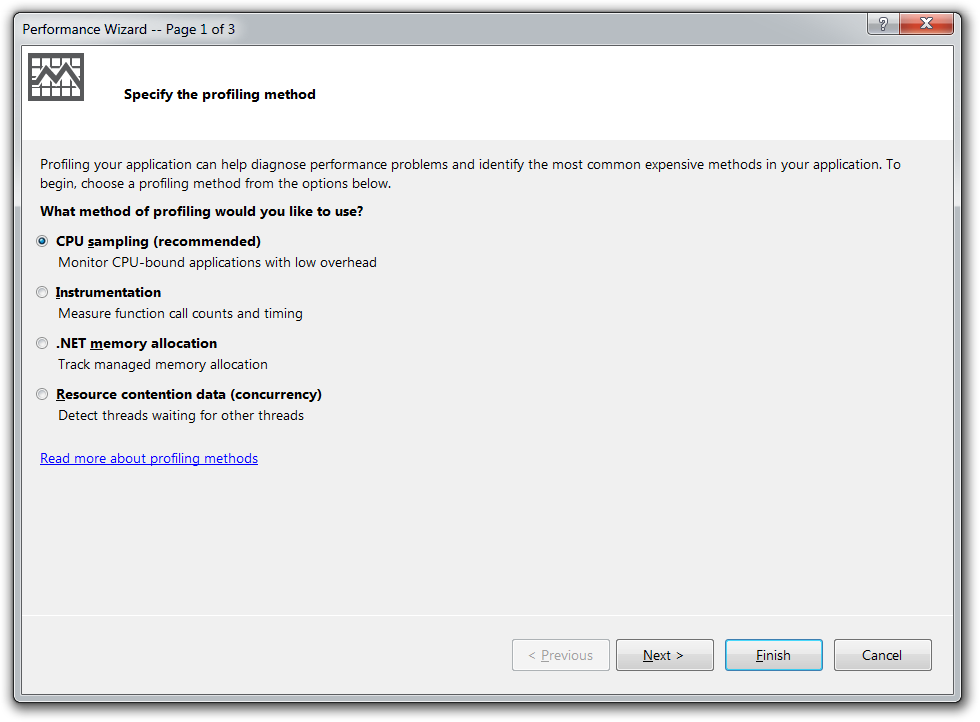
\includegraphics[scale=0.50]{figures/profiler/performance-wizard}
	\caption{De Performance Wizard}
	\label{performance-wizard}
\end{figure}

Wanner het programma klaar is met uitvoeren, worden de resultaten geanalyseerd.
Als dat klaar is, krijg je een algemeen overzicht van de resultaten.
Eerst en vooral zie je een grafiek met het CPU-gebruik doorheen de uitvoeringstijd van de applicatie.
Daaronder zie je de \emph{Hot Paths}, dat zijn de functies die verantwoordelijk zijn voor het grootste deel van de uitvoeringstijd.
Waar wij in geïnteresseerd zijn is hieraan gerelateerd: de \emph{Call Tree View}.
Die geeft je een boomstructuur van functies die elkaar oproepen en enkele belangrijke statistieken:
hoeveel keer een functie werd opgeroepen en hoeveel tijd de functie gemiddeld nodig had om uit te voeren,
dit zowel procentueel (ten opzichte van de totale uitvoeringstijd) als in absolute tijd.

De call tree van de SNMP Data Retriever kun je zien in \cref{call-tree}.
Hierbij werd de \emph{Main} functie opengeklapt. %TODO: Koppelteken
Je kunt functies verder open klappen om te zien welke andere functies worden opgeroepen en hun aandeel in de uitvoeringstijd analyseren.
Dit kan verder gaan tot je atomaire functies krijgt die geen andere functies meer oproepen.

In de call tree zie je naast de functienaam een aantal verschillende kolommen. Hieronder volgt de lijst van de kolommen en hun betekenis.

\begin{itemize}
	\item \textbf{Number of calls:}
		dit spreekt voor zichzelf. Dit is het aantal keren dat een functie opgeroepen werd.
	\item \textbf{Elapsed Inclusive Time \%:}
		dit is het percentage van de uitvoeringstijd dat werd gespendeerd in deze functie en haar kinderen.
	\item \textbf{Elapsed Exclusive Time \%:}
		dit is het percentage van de uitvoeringstijd dat uitsluitend in deze functie werd gespendeerd, dus \emph{exclusief} haar kinderen.
	\item \textbf{Avg Elapsed Inclusive Time:}
		dit is de gemiddelde uitvoeringstijd in milliseconden van deze functie en haar kinderen.
	\item \textbf{Avg Elapsed Exclusive Time:}
		dit is de gemiddelde uitvoeringstijd in milliseconden van uitsluitend deze functie, dus weer \emph{exclusief} haar kinderen.
		\todo{Check of er geen pagebreak is op de individuele items.}
\end{itemize}

\begin{figure}[h]
	\centering
	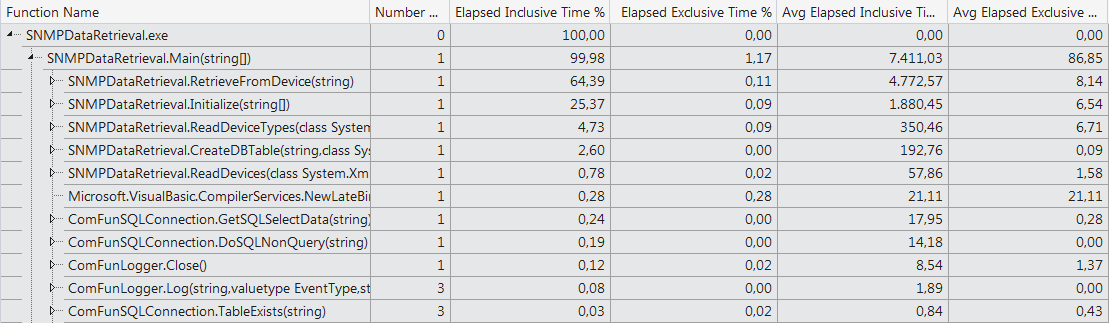
\includegraphics[scale=0.50]{figures/profiler/call-tree}
	\caption[De Call Tree]{De Call Tree. De kolommen van links naar rechts:
		\emph{Function Name},
		\emph{Elapsed Inclusive Time \%},
		\emph{Elapsed Exclusive Time \%},
		\emph{Avg Elapsed Inclusive Time},
		\emph{Avg Elapsed Exclusive Time}.}
	\label{call-tree}
\end{figure}

\subsubsection{Meetresultaten}

Bij dit experiment is het nodig dat we de \nwmretriever{} lokaal uitvoeren en dus niet meer in een virtuele machine.
Voor het wegschrijven van de resultaten installeren we een MariaDB-databank, maar MySQL is ook een optie.

We doen een walk van twee \glspl{oid} op een enkele productieswitch.
Dit zal ons 443 objecten opleveren, waarvan 441 die voor ons relevant zijn.
Volgens de profiler doet de retriever daar ongeveer 7,4 seconden over.
De call tree van de retriever hebben we voor de leesbaarheid in een tabel gegoten (zie \cref{call-tree-main}).
De functies met een extreem kleine uitvoeringstijd (minder dan 0,01\%) hebben we achterwege gelaten.
De kolommen die je ziet zijn de functie, het aantal oproepen, de \emph{inclusieve} tijd als percentage van de totale uitvoeringstijd en
de gemiddelde \emph{inclusieve} tijd in milliseconden.

Voor een globaal overzicht van de werking van de \nwmretriever{} verwijzen we naar \cref{werking}.

% Loglevel 2
\begin{table}[h]
	\centering
	\begin{tabular}{@{}lrrr@{}}
		\toprule
		Functie                                                  & Calls & Tijd (\%) & Tijd (ms) \\ \midrule
		SNMPDataRetrieval.RetrieveFromDevice                     & 1     & 64,39     & 4.772,57  \\
		SNMPDataRetrieval.Initialize                             & 1     & 25,37     & 1.880,45  \\
		SNMPDataRetrieval.ReadDeviceTypes                        & 1     & 4,73      & 350,46    \\
		SNMPDataRetrieval.CreateDBTable                          & 1     & 2,60      & 192,76    \\
		SNMPDataRetrieval.ReadDevices                            & 1     & 0,78      & 57,86     \\
		Microsoft.VisualBasic.CompilerServices.NewLateBinding.L… & 1     & 0,28      & 21,11     \\
		ComFunSQLConnection.GetSQLSelectData                     & 1     & 0,24      & 17,95     \\
		ComFunSQLConnection.DoSQLNonQuery                        & 1     & 0,19      & 14,18     \\
		ComFunLogger.Close                                       & 1     & 0,12      & 8,54      \\
		ComFunLogger.Log                                         & 3     & 0,08      & 1,89      \\
		ComFunSQLConnection.TableExists                          & 3     & 0,03      & 0,84      \\ \bottomrule
	\end{tabular}
	\caption{De call tree van de Main methode} %TODO: Koppelteken
	\label{call-tree-main}
\end{table}

\subsubsection{RetrieveFromDevice-methode}

We beginnen met de functie die het meeste tijd in beslag neemt: de \emph{RetrieveFromDevice}-functie.
Zoals de naam al insinueert, gaat het hier om de methode die de requests stuurt om de gevraagde gegevens op te halen van de verschillende toestellen.

\todo[inline]{Hoort de uitleg over de werking van de SNMP Data Retriever hier?}

De methode werkt als volgt: voor elk toestel dat ondervraagd moet worden,
wordt er een aparte thread gestart, met een maximum van 50 threads.
Elk van die threads zal alle gegevens opvragen die opgevraagd moeten worden voor dat toesteltype
(zie de configuratie van de \nwmretriever{} in \cref{snmp-data-retriever-configuratie}).
Wanneer een thread klaar is met gegevens opvragen, wordt de thread verwijderd.
Indien er nog toestellen zijn die moeten ondervraagd worden, zal er een nieuwe thread opgestart worden voor het volgende toestel.
Dit gaat zo door tot alle toestellen zijn ondervraagd.

In \cref{snmp-operaties} werden de verschillende SNMP operaties besproken waarmee men
gegevens kan opvragen. De originele versie van de SNMP Data Retriever die we eerst testen, maakt gebruik van
GET-requests voor enkelvoudige gegevens en GETNEXT-requests om een SNMP walk te doen van 
een volledige deelboom.

De call tree van de RetrieveFromDevice-functie zie je in \cref{call-tree-retrievefromdevice}.
De twee belangrijkste methoden hier zijn de \emph{SyncRequest} en de \emph{InsertResultRow}-methoden.
SyncRequest maakt deel uit van de \emph{SnmpSource} bibliotheek. %TODO: Koppelteken
Dit is de third party bibliotheek waarvan gebruik gemaakt wordt om alle SNMP interacties af te handelen. %TODO: Koppelteken
De SyncRequest methode wordt gebruikt om synchroon een request te versturen.
Het feit dat de request synchroon gebeurt wil zeggen dat de code wacht op het antwoord alvorens verder te gaan.
We zien dat de methode 443 keer is opgeroepen: er zijn dus 443 requests verstuurd geweest.
Gemiddeld deed een request er een kleine 10 milliseconden over, allen samen goed voor bijna 60\% (oftewel 4,28 seconden) van de totale uitvoeringstijd.

\begin{table}[h]
	\centering
	\begin{tabular}{@{}lrrr@{}}
		\toprule
		Functie                                                  & Calls & Tijd (\%) & Tijd (ms) \\ \midrule
		SnmpSource.SnmpSession.SyncRequest                       & 443   & 57,74     & 9,66      \\
		SNMPDataRetrieval.InsertResultRow                        & 441   & 3,75      & 0,63      \\
		SnmpSource.SnmpSession..ctor                             & 1     & 1,85      & 137,38    \\
		Microsoft.VisualBasic.CompilerServices.NewLateBinding.L… & 445   & 0,42      & 0,07      \\
		ComFunSQLConnection.TableContainsColumn                  & 2     & 0,12      & 4,43      \\
		ComFunLogger.Log                                         & 451   & 0,07      & 0,01      \\
		SnmpSource.SnmpPdu..ctor                                 & 1     & 0,05      & 3,84      \\
		Microsoft.VisualBasic.CompilerServices.Conversions.ToBo… & 2     & 0,04      & 1,59      \\
		Microsoft.VisualBasic.CompilerServices.NewLateBinding.L… & 6     & 0,04      & 0,52      \\
		SnmpSource.SnmpVariable.CreateSnmpVariable               & 443   & 0,02      & 0,00      \\ \bottomrule
	\end{tabular}
	\caption{De call tree van de RetrieveFromDevice methode} %TODO: Koppelteken
	\label{call-tree-retrievefromdevice}
\end{table}

Het versturen van de GETNEXT-requests en het wachten op de antwoorden voor de SNMP walkopdrachten zijn dus
verantwoordelijk voor meer dan de helft van de totale uitvoeringstijd.
Rekening houdend met de resultaten uit \cref{bulkrequests-benchmarks} waarbij GETBULK-requests vier keer sneller gingen dan GETNEXT-requests,
was de keuze dan ook snel gemaakt om de SNMP walkopdracht te implementeren met behulp van GETBULK-requests.

Na het implementeren van de SNMP walkopdracht met behulp van GETBULK-requests doen we een test op basis van dezelfde twee \glspl{oid} als hierboven.
Zoals we in \cref{bulkrequests-benchmarks} beslist hebben, vragen we 50 objecten per request.
We vergelijken de resultaten in \cref{tabel-nwmretriever-met-bulkrequests}.

\begin{table}[h]
\centering
\begin{tabular}{@{}lrrr@{}}
\toprule
                                                                                                 & Uitvoeringstijd (s) & Objecten/ms \\ \midrule
SNMP Walk met GETNEXT-requests                                                                   & 7,371               & 0,064       \\
SNMP Walk met GETBULK-requests (50)                                                              & 3,131               & 0,141       \\
\begin{tabular}[c]{@{}l@{}}RetrieveFromDevice-methode met\\   GETNEXT-requests\end{tabular}      & 5,060               & 0,093       \\
\begin{tabular}[c]{@{}l@{}}RetrieveFromDevice-methode met\\   GETBULK-requests (50)\end{tabular} & 0,722               & 0,611       \\ \bottomrule
\end{tabular}
\caption{SNMP Walk op basis van GETNEXT-requests versus GETBULK-requests in de \nwmretriever{}}
\label{tabel-nwmretriever-met-bulkrequests}
\end{table}

De eerste twee rijen geven de totale uitvoeringstijd weer van de \nwmretriever{},
de laatste twee tonen de uitvoeringstijd van enkel de RetrieveFromDevice-methode gemeten met de profiler.

We zien dat de gemiddelde uitvoeringstijd met ruim vier seconden ingekort wordt, goed voor een ruime verdubbeling van de snelheid.
Als we echter enkel kijken naar de RetrieveFromDevice-methode, zien we dat de methode zelf zeven keer sneller is
geworden dankzij het gebruik van BULK-requests.

\todo[inline]{Vergelijken met de theoretische resultaten? (Adhv. testen met VirtualBox \& iMinds Switchen)}

\begin{table}[h]
\centering
\begin{tabular}{@{}lrrr@{}}
\toprule
Functie                                                  & Calls & Tijd (\%) & Tijd (ms) \\ \midrule
SnmpSource.SnmpSession.SyncRequest                       & 11    & 11,07     & 33,62     \\
SNMPDataRetrieval.InsertResultRow                        & 441   & 6,46      & 0,49      \\
Microsoft.VisualBasic.CompilerServices.NewLateBinding.L… & 1.768 & 1,79      & 0,03      \\
SnmpSource.SnmpSession..ctor                             & 1     & 0,58      & 19,50     \\
Microsoft.VisualBasic.CompilerServices.NewLateBinding.L… & 443   & 0,58      & 0,04      \\
SNMPDataRetrieval.GetRequestsForDevice                   & 1     & 0,34      & 11,22     \\
SnmpSource.SnmpPdu..ctor                                 & 1     & 0,11      & 3,72      \\
Microsoft.VisualBasic.CompilerServices.Conversions.ToBo… & 441   & 0,10      & 0,01      \\
ComFunLogger.Log                                         & 1     & 0,05      & 1,64      \\
System.Array.Exists                                      & 6     & 0,05      & 0,27      \\
SnmpSource.SnmpVariable.CreateSnmpVariable               & 11    & 0,04      & 0,13      \\ \bottomrule
\end{tabular}
\caption{De call tree van de RetrieveFromDevice methode met GETBULK-requests}
\label{call-tree-retrievefromdevice-bulk}
\end{table}

In \cref{call-tree-retrievefromdevice-bulk} zie je hoe de call tree van de RetrieveFromDevice methode er met de nieuwe implementatie uitziet.
Nu doen de SyncRequest oproepen er drie keer zo lang over,
maar er moeten maar 11 requests meer verstuurd worden in plaats van 443.
Twee derde van de uitvoeringstijd van de RetrieveFromDevice-methode wordt besteed aan het ophalen van de gegevens en een derde aan het wegschrijven ervan.
De requests zelf zijn nu nog maar voor 11\% i.p.v. 58\% verantwoordelijk voor de totale uitvoeringstijd.

\begin{table}[h]
\centering
\begin{tabular}{@{}lrrr@{}}
\toprule
Functie                                                  & Calls & Tijd (\%) & Tijd (ms) \\ \midrule
SNMPDataRetrieval.Initialize                             & 1     & 55,57     & 1.857,07  \\
SNMPDataRetrieval.RetrieveFromDevice2                    & 1     & 21,62     & 722,49    \\
SNMPDataRetrieval.ReadDeviceTypes                        & 1     & 12,03     & 401,84    \\
SNMPDataRetrieval.CreateDBTable                          & 1     & 5,31      & 177,32    \\
SNMPDataRetrieval.ReadDevices                            & 1     & 1,39      & 46,56     \\
ComFunSQLConnection.DoSQLNonQuery                        & 1     & 0,79      & 26,49     \\
ComFunSQLConnection.GetSQLSelectData                     & 1     & 0,52      & 17,33     \\
Microsoft.VisualBasic.CompilerServices.NewLateBinding.L… & 1     & 0,47      & 15,71     \\
ComFunLogger.Close                                       & 1     & 0,22      & 7,40      \\
ComFunLogger.Log                                         & 3     & 0,20      & 2,23      \\
ComFunSQLConnection.TableExists                          & 3     & 0,06      & 0,72      \\ \bottomrule
\end{tabular}
\caption{De call tree van de Main methode met GETBULK-requests}
\label{call-tree-main-bulk}
\end{table}

De call tree van de Main-methode met de nieuwe implementatie zien we in \cref{call-tree-main-bulk}.
De retrievalmethode die gebruik maakt van GETBULK-requests hebben we in een andere methode gestoken die de originele vervangt: RetrieveFromDevice2.
De methode die zowel de gegevens ophaalt als wegschrijft is nu nog verantwoordelijk voor minder dan 22\% i.p.v. ruim 64\% van de totale uitvoeringstijd
en is zoals eerder gezegd zeven keer sneller dan de vorige implementatie.

De InsertResultRow-methode in de RetrieveFromDevice-methode hebben we nog niet bekeken.
Die is verantwoordelijk voor het wegschrijven van een gegeven in de databank.
Omdat er 441 gegevens zijn die binnen de SNMP walk vallen, werd de methode 441 keer opgeroepen.

Eén gegeven per keer in de databank wegschrijven klinkt even inefficiënt als het ophalen van één gegeven per keer.
Ook het invoegen van gegevens in een databank kan in bulk gebeuren met behulp van een zogeheten \textit{bulk insert} in plaats van een gewone \textit{insert}.
Hierbij worden de gegevens als één geheel in de databank ingevoerd.
Het voordeel daarbij is dat er zoveel mogelijk gegevens samengebundeld worden in pakketten, waardoor er minder tijd nodig is om alle gegevens te versturen.
De databank hoeft ook maar één query te verwerken in plaats van één voor elk gegeven.

Als we kijken naar de tijd die nodig is om alle gegevens in de databank weg te schrijven, zien we dat
dit slechts iets meer dan 200 ms of 6,5\% van de totale uitvoeringstijd vereist.
We beslissen dan ook dat het niet de moeite is om dit te implementeren, omdat er elders nog veel grotere winsten kunnen gehaald worden\footnote{
	Wat we echter over het hoofd hebben gezien is dat we de lokale databankinstallatie geïnstalleerd hebben op een SSD.
	Een databank heeft enorm veel baat bij het gebruik van een SSD door de lage \textit{random access} tijd en heeft weinig moeite om een groot aantal inserts bij te houden zoals onze test.
	Pas bij de grootschalige tests ontdekken we onze fout, en daar komen we er dan ook op terug.
}.


\subsubsection{Initialize-methode}

Als we de call tree van de Main-methode bekijken, dan valt het op dat er naast de RetrieveFromDevice-methode,
die logischerwijs een belangrijke factor is in de uitvoeringstijd,
nog een methode is die voor een groot stuk medeverantwoordelijk is voor de uitvoeringstijd: de \textit{Initialize}-methode.

In de originele implementatie was die verantwoordelijk voor 25\% van de uitvoeringstijd, in de nieuwe is dit opgelopen tot bijna 56\%!
De Initialize-methode doet er bijna 2 seconden over.
Bijgevolg zijn we erg niewsgierig wat er juist in deze methode gebeurt waardoor deze zoveel tijd nodig heeft.
We beginnen met het analyseren van de call tree van de functie, te zien in \cref{call-tree-initialize}.
Wat we zien zijn twee oproepen naar een \emph{Log}-methode die er gemiddeld bijna een seconde over doet \emph{per oproep}! %TODO: Koppelteken

\begin{table}[h]
\centering
\begin{tabular}{@{}lrrr@{}}
\toprule
Functie                                                   & Calls & Tijd (\%) & Tijd (ms) \\ \midrule
ComFunLogger.Log                                          & 2     & 45,61     & 762,05    \\
ComFunSQLConnection..ctor                                 & 1     & 8,15      & 272,18    \\
ComFunLogger.set\_LogFile                                 & 1     & 0,42      & 14,17     \\
Microsoft.VisualBasic.CompilerServices.Conversions.ToIn…  & 2     & 0,32      & 5,41      \\
ComFunLogger.Log                                          & 4     & 0,29      & 2,44      \\
System.Configuration.ConfigurationManager.get\_AppSettin… & 12    & 0,22      & 0,61      \\
ComFunLogger.Log                                          & 3     & 0,13      & 1,46      \\
ComFunLogger.Log                                          & 2     & 0,10      & 1,73      \\
ComFun.NetworkMiningCopyRightStatement                    & 1     & 0,06      & 2,14      \\
ComFunLogger..ctor                                        & 1     & 0,03      & 1,07      \\ \bottomrule
\end{tabular}
\caption{De call tree van de Initialize methode} %TODO: Koppelteken
\label{call-tree-initialize}
\end{table}

De \emph{ComFunLogger} is een stuk code die gebruikt wordt om te loggen naar een tekstbestand.
De naam komt van het feit dat ze een gemeenschappelijk stuk code is die over meerdere projecten kan
gebruikt worden: \emph{common functions}, of \emph{ComFun} voor kort.
Maar een functie die loggegevens wegschrijft naar een bestand zou niet zo lang mogen duren.
I/O-operaties zijn kostelijk, maar niet in die mate. %TODO: Koppelteken
Als we de functie helemaal openklappen in \cref{call-tree-performancecounter}, vinden we de echte dader:
een constructor van \emph{System.Diagnostics.PerformanceCounter}.
Een performance counter wordt gebruikt voor het monitoren van systeemcomponenten zoals
processoren, geheugen en netwerk-I/O. Als je counters gebruikt in je applicatie kunnen ze je %TODO: Koppelteken
informatie geven over de performantie van je programma.\cite{performance-counters-intro}
De ComFunLogger gebruikt ze om het geheugengebruik te meten en weg te schrijven in de logbestanden.

\begin{figure}[h]
	\centering
	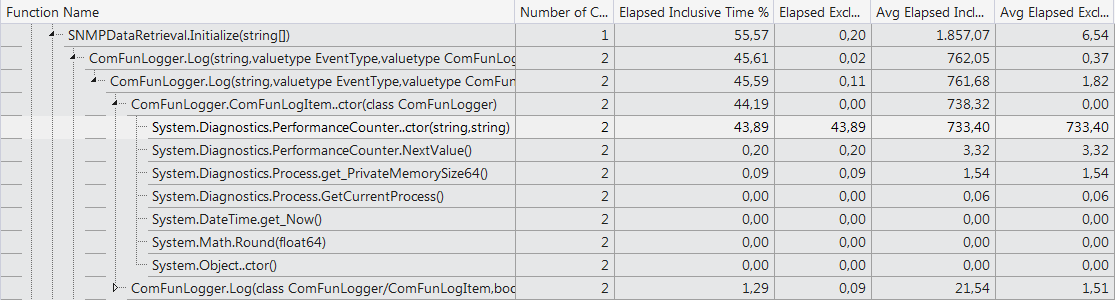
\includegraphics[scale=0.50]{figures/profiler/call-tree-performancecounter}
	\caption{De call tree van de Log methode}
	\label{call-tree-performancecounter}
\end{figure}

\todo[inline]{Herlees mij.}

Als oplossing werd ervoor gekozen om een alternatief \emph{logging framework} te gebruiken.
Dit lijkt een drastische maatregel (en dat is het ook), maar daar zijn goede redenen voor.
De noodzaak aan een tool om informatie te loggen is een algemeen probleem.
Er zijn dan ook een heleboel gratis en open-source logging frameworks die reeds hun nut en kunnen bewezen hebben.
Ontwikkelaars doen er goed aan om deze bestaande tools te hergebruiken in hun projecten.

Financiëel is het een goede keuze want de software is al ontwikkeld en werd al grondig getest door vele anderen.
Dit spaart tijd en geld uit voor de ontwikkeling van een eigen oplossing.
De software is gratis in gebruik: er zijn geen licentiekosten aan verbonden.
Er zijn ook geen of lage onderhoudskosten.

Ook vanuit het technisch perspectief is het een goede keuze.
Omdat de software reeds ingezet wordt in verschillende projecten werd ze zo flexibel mogelijk gemaakt en bevat ze reeds een resem aan extra functionaliteit.
Zo kan je loggen naar meerdere outputs en zijn er meerdere mogelijke outputs beschikbaar.
Je kunt bijvoorbeeld loggen naar tekstbestanden, consolevensters, databanken, enzovoort.
Mocht er toch iets toegevoegd dienen te worden, dan beschik je over de broncode om dit gemakkelijk zelf te kunnen doen.

De twee belangrijkste redenen echter zijn het feit dat ze ontwikkeld zijn om een zo klein mogelijke performantieimpact te hebben en
dat de integratie ervan in een project zeer eenvoudig is.
Zo was het veel sneller om een ander logging framework te gebruiken dan om de bestaande loggingcode te doorspitten op zoek naar problemen en mogelijke optimalisaties.

De keuze uit de verschillende logging frameworks is uiteindelijk gevallen op Apache log4net.
Deze is gebaseerd op het waarschijnlijk bekendste logging framework voor Java: Apache log4j.
Bij de keuze werd rekening gehouden met de performantieimpact en de features van de verschillende logging frameworks.\footnote{
	Een vergelijking tussen de bekendste logging frameworks voor .NET vind je 
	terug in de bronnenlijst bij bron \cite{logging-frameworks-and-performance} en \cite{logging-frameworks}.
}

Net als bij het implementeren van GETBULK-requests laten we opnieuw de \nwmretriever{} dezelfde \glspl{oid} opvragen van een productieswitch.
We vergelijken de resultaten met de vorige testen in \cref{tabel-nwmretriever-met-bulkrequests-en-log4net}.
Om zicht te hebben op de overhead van de \nwmretriever{} bekijken we ook de performantie van enkel de RetrieveFromDevice-methode (ophalen en wegschrijven in databank) en alle SyncRequest-methoden samen (enkel het ophalen van de gegevens).
Ten slotte vergelijken we ook met de resultaten die we in het verleden behaalden met Net-SNMP bij het bevragen van dezelfde switch.
Toen ging het wel om een pak meer gegevens: ongeveer 2750 tegenover ongeveer 441 hier.

\begin{table}[h]
\centering
\begin{tabular}{@{}lrrr@{}}
\toprule
                                                                                                 & Uitvoeringstijd (s) & Objecten/ms \\ \midrule
SNMP Walk met GETNEXT-requests                                                                   & 7,371               & 0,064       \\
SNMP Walk met GETBULK-requests (50)                                                              & 3,131               & 0,141       \\
\begin{tabular}[c]{@{}l@{}}SNMP Walk met GETBULK-requests en\\   log4net (50)\end{tabular}       & 1,839               & 0,240       \\
\begin{tabular}[c]{@{}l@{}}RetrieveFromDevice-methode met\\   GETBULK-requests (50)\end{tabular} & 0,722               & 0,611       \\
\begin{tabular}[c]{@{}l@{}}SyncRequest-methode met GETBULK-requests\\   (50)\end{tabular}        & 0,387               & 1,138       \\
Net-SNMP Bulkwalk (50)                                                                           & 1,488               & 1,848       \\ \bottomrule
\end{tabular}
\caption{Vergelijking van de verschillende implementaties van \nwmretriever{} en Net-SNMP}
\label{tabel-nwmretriever-met-bulkrequests-en-log4net}
\end{table}

Opnieuw zien we een grote verbetering: de uitvoeringstijd is nu 1,7 keer sneller ten opzichte van de vorige versie,
en vier keer sneller dan de originele versie!
Alhoewel we zeer grote performantiewinsten behaald hebben ten opzichte van de originel versie van de \nwmretriever{},
als we enkel kijken naar het ophalen van de gegevens door de SyncRequest-methode,
dan is dit nog steeds 38\% trager dan bij Net-SNMP.
Maar omdat deze methode onderdeel is van de third-party bibliotheek SnmpSource kunnen we daar verder geen verbeteringen meer aanbrengen.

\begin{table}[]
\centering
\begin{tabular}{@{}lrrr@{}}
\toprule
Functie                                                  & Calls & Tijd (\%) & Tijd (ms) \\ \midrule
SNMPDataRetrieval.RetrieveFromDevice2                    & 1     & 38,80     & 725,19    \\
SNMPDataRetrieval.ReadDeviceTypes                        & 1     & 17,20     & 321,51    \\
SNMPDataRetrieval.Initialize                             & 1     & 17,02     & 318,13    \\
log4net.Config.XmlConfigurator.Configure                 & 1     & 10,25     & 191,52    \\
SNMPDataRetrieval.CreateDBTable                          & 1     & 8,28      & 154,77    \\
SNMPDataRetrieval.ReadDevices                            & 1     & 2,50      & 46,77     \\
ComFunSQLConnection.GetSQLSelectData                     & 1     & 0,95      & 17,75     \\
Microsoft.VisualBasic.CompilerServices.NewLateBinding.L… & 1     & 0,87      & 16,26     \\
ComFunSQLConnection.DoSQLNonQuery                        & 1     & 0,75      & 14,02     \\
log4net.LogManager.GetLogger                             & 1     & 0,44      & 8,14      \\
ComFunSQLConnection.TableExists                          & 3     & 0,12      & 0,76      \\
log4net.ILog.Info                                        & 3     & 0,06      & 0,39      \\ \bottomrule
\end{tabular}
\caption{De call tree van de Main methode met GETBULK-requests en log4net}
\label{call-tree-main-bulk-en-log4net}
\end{table}

De call tree van de Main-methode van de nieuwste versie zie je in \cref{call-tree-main-bulk-en-log4net}.
De totale uitvoeringstijd wordt nu voornamelijk bepaald door de volgende onderdelen:

\begin{itemize}
	\item 38,80\% (725 ms): het bevragen van het toestel en het wegschrijven van de gegevens in de databank.
	\item 17,20\% (322 ms): het inlezen van de toesteltypes uit het XML-configuratiebestand.
		Het gebruik van reguliere expressies heeft hier de meeste impact op.
	\item 17,02\% (318 ms): het initialiseren,
		de meeste tijd wordt hier besteed aan de constructie van een SQL \textit{Connection}-object (250 ms).
	\item 10,25\% (192 ms): het inlezen van het log4net-configuratiebestand.
	\item 8,28\% (155 ms): het aanmaken van de databanktabellen.
	\item 2,50\% (47 ms): het inlezen van de te bevragen toestellen uit het XML-configuratiebestand.
\end{itemize}

\subsubsection{Conclusie}

Het implementeren van de SNMP walkopdracht met behulp van GETBULK-requests en het vervangen van het logging framework
door log4net heeft ervoor gezorgd dat de \nwmretriever{} vier keer sneller werkt in vergelijking met de originele versie.
Alhoewel we het hier niet bekeken hebben, is er nog een optimalisatiemogelijkheid bij het wegschrijven van de gegevens in de databank.
Daar kunnen de gegevens best in bulk weggeschreven worden in plaats van gegeven per gegeven zoals nu.

\todo[inline, caption={}]{

\begin{itemize}
	\item Waarom zijn er twee instanties nodig van de PerformanceCounter?
	\item Onderzoek op het internet leert ons dat PerformanceCounters hele kostelijke objecten zijn om aan te maken. Bron/citaat?
	\item x Oplossing: alternatieve loggingframework. Maar waarom heb je hiervoor gekozen ipv de huidige aan te passen?
	\item x Performantieredenen: ik heb een tried \& true logging framework opgezocht met nadruk op een minimale performantieimpact.
	\item x Plus de implementatie is ook sneller. Dan moet ik niet mijzelf bekend maken met de oude loggingcode en heb ik maar het 
		nieuwe loggingframework te includeren en alle logcalls te vervangen, wat vrij snel gebeurd is.
	\item x Lagere onderhoudskosten
	\item x Geen licentiekosten
	\item x Als leuke bonus krijg je er ook een heleboel extra features bij zoals logging naar meerdere outputs en meer outputformaten. (extra flexibiliteit)
	\item x Denk aan textfile, XML file, DB file, consoleuitvoer, etc.
	\item Nadeel: hoe groot is de extra code/binary van dit loggingframework? Andere nadelen?
\end{itemize}

}

\subsection{Tabellen rij per rij opvragen i.p.v. kolom per kolom}
\label{rij-per-rij}
\todo[inline]{Betere/kortere titel?}

Zoals uitgelegd in \cref{snmp-tabellen} worden tabellen kolom per kolom overlopen bij een SNMP walkopdracht.
Een meer natuurlijke manier van werken zou zijn om de tabel rij per rij op te vragen.
En misschien valt die methode zelfs sneller uit.

Een gewone SNMP walk wordt geïmplementeerd door GETNEXT-requests (of GETBULK-requests)
en vraagt zo steeds de volgende \gls{oid} op.
Om een tabel rij per rij op te vragen, moeten we de opeenvolgende kolommen van de eerste rij opvragen, gevolgd door de kolommen van de tweede enzovoort.
Maar het kan nog sneller: we kunnen meteen alle kolommen van de eerste rij opvragen, gevolgd door alle kolommen van de tweede rij enzovoort.
Om dat te doen kunnen we een GETNEXT-request opstellen met de \glspl{oid} van alle kolommen van een tabel.
Een GETNEXT-request geeft ons dan de kolommen terug van de eerste rij en zo weten we meteen ook de index waarmee we de volgende request kunnen samenstellen.
Dat geeft ons dan de kolommen van de tweede rij en zo gaan we verder tot we de volledige tabel hebben opgehaald.

Jammer genoeg is het niet voldoende om met Net-SNMP een snmpbulkwalk te doen met de \glspl{oid} van alle kolommen want
die doet simpelweg sequentieel een snmpbulkwalk van elke opgegeven \gls{oid}.
Dus moeten we het wiel heruitvinden, en een snmpbulkwalk implementeren die wel alle \glspl{oid} in parallel overloopt en op het juiste moment stopt.

Daarvoor maken we gebruik van GETBULK-requests met de \glspl{oid} van alle kolommen.
Door het aantal herhalingen in te stellen kunnen we meteen ook meerdere rijen tegelijkertijd opvragen.
Het aantal max-repetitions is dan gelijk aan het aantal rijen dat in een request wordt opgevraagd.
Om het aantal objecten in een request te weten te komen, vermenigvuldig je simpelweg het aantal max-repetitions met het aantal kolommen.

Om op het juiste moment te stoppen moeten we ofwel op voorhand het aantal rijen kennen, ofwel moeten we de teruggegeven \glspl{oid}
bekijken om te zien of ze nog steeds deel uitmaken van de tabel, zoals een gewone SNMP walk doet.

De voorwaarde om dit alles te kunnen doen, is dat we vooraf de \glspl{oid} van de kolommen van de tabel kennen.
Om de snelheid te vergelijken tussen beiden manieren om een tabel te overlopen,
bepalen we het maximum aantal rijen dat we tegelijkertijd kunnen opvragen, zodat het aantal objecten in een request onder 50 blijft.
Dan overlopen we de tabel met een gewone SNMP walk op basis van GETBULK-requests met hetzelfde aantal objecten in een request.

Een voorbeeld: de interfacetabel ifTabel heeft 22 kolommen, dus dan vragen we 2 rijen per request op (goed voor 44 objecten per request).
Bij de gewone snmpbulkwalk geven we dan als aantal max-repetitions 44 op zodat beide methoden evenveel objecten per request opvragen.

\subsubsection{Meetresultaten}

Om te beginnen vragen we de dot1dBasePortTable (1.3.6.1.2.1.17.1.4) op van de productieswitches bij iMinds.
Vanwege de problemen bij het genereren van grote hoeveelheden verkeer (\cref{probleem-dos-bescherming}) konden we slechts één iteratie per keer uitvoeren.
Alhoewel we de test meermaals hebben herhaald om zeker te zijn dat er geen grote verschillen zijn in de metingen,
is het toch belangrijk om in het achterhoofd te houden dat de resultaten niet erg nauwkeurig zijn.

\todo[inline]{Aantal objecten/ms? Niet echt interessant vermits we zo weinig metingen hebben...}

\begin{table}[h]
\centering
\begin{tabular}{@{}lrrr@{}}
\toprule
Toestel  & Objecten & Uitvoeringstijd rij per rij (s) & Uitvoeringstijd kolom per kolom (s) \\ \midrule
atlas1a1 & 1315     & 1,09                            & 0,59                                \\
atlas2a1 & 615      & 0,36                            & 0,25                                \\
atlas2a2 & 250      & 0,37                            & 0,28                                \\
atlas3a1 & 250      & 0,32                            & 0,21                                \\ \bottomrule
\end{tabular}
\caption{Tabel rij per rij opvragen versus kolom per kolom}
\label{tabel-serieel-vs-parallel}
\end{table}

Ondanks de minder nauwkeurige resultaten in \cref{tabel-serieel-vs-parallel} kunnen we wel een algemene trend waarnemen:
de tabel kolom per kolom ophalen is gemiddeld ongeveer de helft sneller dan ze rij per rij op te halen.
Deze trend zien we ook bij de andere productieswitches.
Voor alle duidelijkheid: deze testen zijn gebaseerd op de Net-SNMP tools.

Naar aanleiding van de grootschalige testen hebben we al een kleine opstelling klaar, die gelijkaardig is aan de virtuele machines qua softwareconfiguratie,
maar waarbij elke machine op een \textit{dedicated server}\footnote{
	Bij een dedicated server worden de resources van een machine volledig toegewijd tot een of meer taken,
	in tegenstelling tot een virtuele machine die slechts een deel van de resources van een toestel krijgt.
} draait.
Omdat deze servers in een apart netwerk zitten hebben we gelukkig geen problemen met het genereren van veel verkeer.
Daar kunnen we zoveel verkeer versturen als de fysieke verbinding aankan.
We kunnen daar dezelfde test doen maar met voldoende herhalingen om een nauwkeuriger resultaat te bekomen.

De ping tijd tussen de twee toestellen is gemiddeld 0,204 ms.
Dat is nog lager dan tussen de virtuele toestellen, die 0,468 ms bedroeg, en ongeveer negen keer lager dan bij de productieswitches van hierboven.
Bij deze test vragen we de interfacetabel ifTable (1.3.6.1.2.1.2.2) op.
De tabel heeft 22 kolommen en de server heeft zes interfaces, samen goed voor 154 objecten.
Omdat 154 objecten wat aan de lage kant is,
kunnen we een aantal VLAN's toewijzen aan interfaces om het aantal objecten te verhogen,
want VLAN's komen ook in de interfacetabel terecht.
Om een VLAN aan te maken gebruik je het volgend commando:

\begin{lstlisting}[caption={Aanmaken van een VLAN}, label=commando-vlan]
$ sudo ip link add link eth3 name eth3.100 type vlan id 100
\end{lstlisting}

Met dit commando wordt het VLAN met ID 100 toegewezen aan interface \textit{eth3} en krijgt die de naam \textit{eth3.100}.
We doen dit voor een 100-tal VLAN's, goed voor 2200 extra objecten of 2354 objecten in totaal in de tabel.

\begin{table}[h]
\centering
\begin{tabular}{@{}lrrr@{}}
\toprule
                & Objecten & Uitvoeringstijd (ms) & Objecten/ms \\ \midrule
Rij per rij     & 154      & 109                  & 1,413       \\
Kolom per kolom & 154      & 30                   & 5,133       \\
Rij per rij     & 2354     & 1523                 & 1,546       \\
Kolom per kolom & 2354     & 80                   & 29,425      \\ \bottomrule
\end{tabular}
\caption{Tabel rij per rij opvragen versus kolom per kolom op dedicated hardware}
\label{tabel-serieel-vs-parallel-vwall}
\end{table}

In \cref{tabel-serieel-vs-parallel-vwall} zien we de resultaten.
Opnieuw is het sneller om een tabel kolom per kolom op te vragen in plaats van rij per rij.
Deze keer is het zelfs ruim drie keer sneller bij 154 objecten.
2354 objecten zijn ongeveer 15 keer meer objecten, en de tabel rij per rij overlopen doet er ook 15 keer langer over.
Bij het kolom per kolom overlopen echter is de uitvoeringstijd amper met een factor drie toegenomen!
We hebben de test (van 100 iteraties) meermaals uitgevoerd om  te bevestigen dat de resultaten kloppen,
maar de metingen bleken zeer consistent.

\todo[inline]{Onderzoek de Wireshark trace.}

Het is duidelijk dat het sneller is om tabellen kolom per kolom op te vragen.
Maar behalve het snelheidsverschil zijn er nog andere redenen om tabellen op die manier te overlopen:

\begin{itemize}
	\item De implementatie bestaat al en is uitvoerig getest.
	\item Voorkennis van de tabel is vereist om een tabel rij per rij te overlopen: er moet dus een goede integratie zijn van de \gls{mib}-bestanden
		om op de kolommen van elke tabel te bepalen en om te weten welke \glspl{oid} overeenstemmen met een tabel.
	\item Als de tabel deel uitmaakt van een SNMP walk van een hoger gelegen \gls{oid},
		dan moet er tijdens de uitvoering van implementatie gewisseld worden bij de \gls{oid} van de tabel, wat extra complexiteit veroorzaakt.
	\item Er moet rekening gehouden worden met randsituaties.
		Zo zou het mogelijk zijn dat er celwaarden in een tabel ontbreken volgens \cite{net-snmp-table-holes}.
		Wij hebben dit echter nooit kunnen vaststellen.
		Bij het rij per rij overlopen zou een antwoordpakket dus al een kolomwaarde kunnen bevatten van de volgende rij!
	\item Het configureren van het aantal objecten dat per request opgehaald moet worden, is niet zo flexibel:
		omdat je enkel het aantal rijen kunt opgeven,
		is het aantal objecten per request automatisch een veelvoud van het aantal kolommen.
\end{itemize}

\subsubsection{Conclusie}

Het rij per rij overlopen van een tabel is niet alleen trager dan ze kolom per kolom te overlopen,
ze brengt ook een groot aantal problemen mee bij de implementatie.
Indien je toch een tabel rij per rij wil \textit{lezen}, dan kan je beter gebruik maken van bijvoorbeeld de Net-SNMP \textit{snmptable} tool.
Deze vraagt een tabel kolom per kolom op zoals gewoonlijk, maar beeldt ze rij per rij af en houdt ook rekening met speciale gevallen zoals gaten in de tabel.


\subsection{Impact van de fragmentatie van pakketten}
\todo{Titel: Snelheidsimpact?}

In dit experiment onderzoeken we de impact van de fragmentatie van pakketten.
Dit doet zich voor als we proberen teveel objecten in een request te steken waardoor ze groter wordt dan de \gls{mtu} en
bijgevolg moet opgesplitst worden in meerdere pakketten alvorens ze verstuurd kan worden.

We trachten om de gemiddelde grootte te bepalen van objecten om een schatting te doen van het ideaal aantal objecten per request
zodat we zo veel mogelijk objecten per request kunnen opvragen maar er toch zo weinig mogelijk fragmentatie voorkomt.
Dit experiment wordt bemoeilijkt omdat de objecten en zelfs de headers van een SNMP-bericht geen vaste grootte hebben.
Om de gemiddelde objectgrootte te bepalen, moeten we een SNMP-bericht volledig ontleden en de grootte van alle headers bepalen.
Eenmaal we de gemiddelde objectgrootte kennen, berekenen we hoeveel objecten er in een niet-gefragmenteerd bericht passen.
Vervolgens meten we hoelang een gefragmenteerd bericht er over doet tegenover een niet-gefragmenteerd bericht,
hoeveel gefragmenteerde berichten er werkelijk zijn in een SNMP walk,
en tenslotte vergelijken we de uitvoeringstijd met een SNMP walk met een ''optimaal'' aantal objecten per request.

\todo[inline]{
Eerst en vooral bekijken we in welke mate fragmentatie zich voordoet bij het aanhouden van 50 objecten per request.
Daarna zullen we de gemiddelde grootte bepalen van objecten om een schatting te doen van het ideaal aantal objecten per request
zodat we zo veel mogelijk objecten per request kunnen opvragen maar en toch zo weinig mogelijk fragmentatie voorkomt.
Tenslotte bekijken we wat voor impact de fragmentatie van pakketten/beide aanpakken hebben op de uitvoeringstijd en vormen we onze conclusie.
}

\subsubsection{Gemiddelde objectgrootte en optimaal aantal objecten per request}

Om de gemiddelde objectgrootte te berekenen, doen we een SNMP walk van de mib-2-tak (1.3.6.1.2.1).
We gebruiken de variant op basis van GETNEXT-requests, zodat elk antwoordbericht juist één object bevat.
Dat levert ons 3560 \emph{antwoord}berichten op.
De gemiddelde lengte van een antwoordbericht bedraagt 102,26 bytes.
Dus nemen we willekeurig een antwoordbericht van 102 bytes om te ontleden.

Om te beginnen hebben we de ethernetheader, goed voor 14 bytes\cite{ethernet-header}.
Daarna volgt de IP-header, typisch van 20 bytes\cite{ipv4-header-wiki}.
Na de IP-header komt de SNMP-\gls{pdu} die de overige 68 bytes ($ 102 - 14 - 20$) voor zijn rekening neemt.

De berichtstructuur van een SNMP-bericht hebben we besproken in \cref{snmp-berichtstructuur}.
Zoals gezegd hebben SNMP-berichten een variable headerlengte.
Maar veel headervelden hebben in de praktijk een vaste lengte.
We overlopen alle velden van een SNMP-header en bepalen hun typische lengte.
Als referentie kun je nogmaals de structuur van een SNMP-bericht bekijken in \cref{fig-berichtstructuur-4}.

\begin{figure}[h]
	\centering
	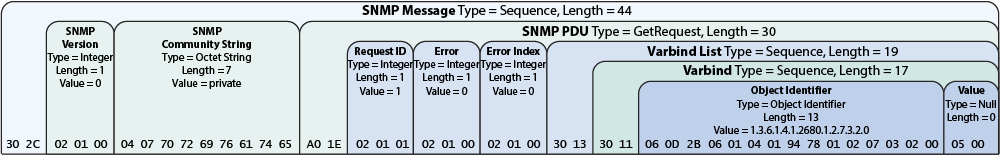
\includegraphics[scale=0.40]{figures/snmp/berichtstructuur-3}
	\caption[Berichtstructuur van een SNMP-bericht in detail]{Berichtstructuur van een SNMP-bericht in detail\cite{snmp-message-format}}
	\label{fig-berichtstructuur-4}
\end{figure}

Het SNMP-bericht is een sequentie van:

\begin{itemize}
	\item De SNMP versie: steeds 1 byte.
	\item De community string: variabel, maar uitgaande van de community ''public'' gaat het om 6 bytes.
	\item De SNMP-\gls{pdu}: bestaat uit:
		\begin{itemize}
			\item De request ID: de unieke identificatie van een request.
				Bij de SNMP walk hadden alle requests de ID 1, dus: 1 byte.
			\item Het errorveld: een byte.
			\item Error Index: staat op nul indien er zich geen fout heeft voorgedaan, dus ook 1 byte.
			\item Varbind List: een sequentie van varbinds, maar bij de SNMP walk op basis van GETNEXT-requests gaat het om slechts een object.
				\begin{itemize}
					\item Varbind: stelt een object voor en is hetgeen we trachten te bepalen
						\begin{itemize}
							\item OID: variabel aantal bytes
							\item Value: variabel aantal bytes
						\end{itemize}
				\end{itemize}
		\end{itemize}
\end{itemize}

In totaal heeft een SNMP-bericht dus 8 vaste \gls{tlv}-tripletten (tot en met de Varbind List) met elk een overhead van 2 bytes voor de tag en length,
wat goed is voor 16 bytes.
De values die een vaste lengte hebben zijn samen goed voor 10 bytes.
Elk object wordt voorgesteld door een Varbind bestaande uit een \gls{oid} en een value, samen goed voor een overhead van 6 bytes per object.
Uiteindelijk komen we uit op een headerlengte van 26 bytes voor het SNMP-bericht zonder objecten.

Als we de headerlengte van 26 bytes aftrekken van de 68 bytes van het SNMP-gedeelte van ons GETNEXT-response houden we nog 42 bytes over voor de varbind
die het object en zijn \gls{oid} en value bevatten.
Een gemiddeld object heeft dus een lengte van 42 bytes, inclusief zijn headers.

We gaan uit van een \gls{mtu} van 1500 bytes voor een ethernetpakket.
Als we daarvan de lengtes aftrekken van de ethernet-, IP- en SNMP-header houden we nog 1440 bytes ($1500 - 14 - 20 - 26$) over voor de objecten en hun headers.
Uitgaande van een gemiddelde objectlengte van 42 bytes is dat goed voor iets meer dan 34 objecten.

\subsubsection{Meetresultaten}

We laten de \nwmretriever{} op basis van de nieuwe implementatie een SNMP walk doen met 34 en 50 objecten.
Met behulp van Wireshark analyseren we de pakketten van beide tests.

We bepalen voor beide tests de impact van de fragmentatie op antwoordberichten door de gemiddelde tijd te meten die de pakketten nodig hebben.
De tijd die een pakket nodig heeft is dan het tijdsverschil tussen het versturen van de request tot het ontvangen van het responsbericht.
We bepalen tenslotte voor beide tests ook het percentage pakketten die gefragmenteerd werden.

\begin{table}[h]
\centering
\begin{tabular}{@{}lrrrrr@{}}
\toprule
                                                                           & Objecten/request & Aantal & Percentage & Tijd (ms) & Tijdsverschil (ms) \\ \midrule
\begin{tabular}[c]{@{}l@{}}Niet-gefragmenteerde\\   pakketten\end{tabular} & 50               & 22     &            & 6,996     &                    \\
\begin{tabular}[c]{@{}l@{}}Gefragmenteerd\\   pakketten\end{tabular}       & 50               & 50     & 69,44\%    & 9,822     & 2,826 (+40,39\%)   \\
\begin{tabular}[c]{@{}l@{}}Niet-gefragmenteerde\\   pakketten\end{tabular} & 34               & 83     &            & 5,843     &                    \\
\begin{tabular}[c]{@{}l@{}}Gefragmenteerd\\   pakketten\end{tabular}       & 34               & 22     & 20,95\%    & 7,882     & 2,039 (+34,9\%)    \\ \bottomrule
\end{tabular}
\caption{Impact en percentage van gefragmenteerde pakketten bij bulkrequests}
\label{tabel-fragmentatie-impact-percentage}
\end{table}

\todo[inline]{\Cref{tabel-fragmentatie-impact-percentage}: is het duidelijk dat het hier om tijd PER PAKKET gaat?}

In \cref{tabel-fragmentatie-impact-percentage} zien we het aantal gefragmenteerde- en niet-gefragmenteerde pakketten bij bulkrequests van 34 en 50 objecten per request.
Ook getoond is de gemiddelde tijd die nodig was om een antwoordbericht te ontvangen en het tijdsverschil tussen de gefragmenteerde- en niet-gefragmenteerde pakketten.
We zien dat bij 50 objecten per request het percentage van pakketten dat gefragmenteerd werd vrij hoog ligt: net geen 70\% en dat ze er ook 40\% langer over doen.
Bij 34 objecten per request is dat percentage sterk gedaald en we zien ook dat de tijd die de pakketten erover doen gedaald is als gevolg van
het kleiner aantal objecten per request.

Maar de vraag is nu of het loont om 32\% minder objecten in een pakket te steken zodat ze 35 à 40\% sneller gaan?
Daarvoor laten we de \nwmretriever{} een SNMP walk doen van de \textit{enterprises}-tak (1.3.6.1.4.1) en de gekende mib-2-tak, samen goed voor 3558 objecten.

\begin{table}[h]
\centering
\begin{tabular}{@{}rrrr@{}}
\toprule
Objecten/request & Objecten & Uitvoeringstijd (s) & Tijdsverschil (s) \\ \midrule
50               & 3558     & 17,735              &                   \\
34               & 3558     & 18,626              & 0,891 (+5,02\%)   \\ \bottomrule
\end{tabular}
\caption{Gemiddelde uitvoeringstijd van een SNMP walk met 50 en 34 objecten per request}
\label{tabel-fragmentatie-uitvoeringstijd}
\end{table}

In \cref{tabel-fragmentatie-uitvoeringstijd} zien we dat de SNMP walk met 34 objecten per request er gemiddeld bijna een seconde (of 5\%) langer over doet
dan de SNMP walk met 50 objecten per request.
Het is duidelijk dat de tijdswinst van niet-gefragmenteerde pakketten niet opweegt tegen de tijdswinst bij het opvragen van meer objecten per request.

\subsubsection{Conclusie}

Ondanks het feit dat we antwoordberichten een stuk sneller krijgen als ze niet gefragmenteerd hoeven te worden,
lijkt die tijdswinst toch niet op te wegen tegen de tijdswinst van het opvragen van meer requests per object.
We kunnen dus beter meer requests per object opvragen, zelfs als dat een hoge mate van fragmentatie veroorzaakt.


\section{Grootschalige benchmarks en experimenten}

\todo[inline]{Inleiding nodig? Reeds uitgelegd in inleiding van het hoofdstuk.}

\subsection{Testopstelling}

\subsubsection{Virtual Wall}

De Virtual Wall is een testomgeving bij iMinds voor geavanceerde netwerken, gedistribueerde software en dienstenevaluatie.
Ze ondersteunt het onderzoek naar de schaalbaarheid van toepassingen.
De Virtual Wall bestaat uit een kleine 200 zware servers met processoren gaande van vier tot twaalf cores,
tot 24 GB geheugen en hebben tot zes gigabit netwerkinterfaces.
De servers zijn verbonden met grote switches die als schakelbord functioneren.
Zo kunnen de servers vanop afstand op elke mogelijke wijze met elkaar verbonden worden.
De servers zelf kunnen ook op afstand voorzien worden van voorgeconfigureerde software images.
Zo kunnen servers geconfigureerd worden als server, klant of zelfs als een netwerkelement.
Op het netwerk kan men ook testen doen met verbindingen die pakketten verliezen, beperkte bandbreedte hebben of
een grote netwerkvertraging ondervinden\cite{virtual-wall-uitleg, virtual-wall-specs}.

\begin{figure}[h]
	\centering
	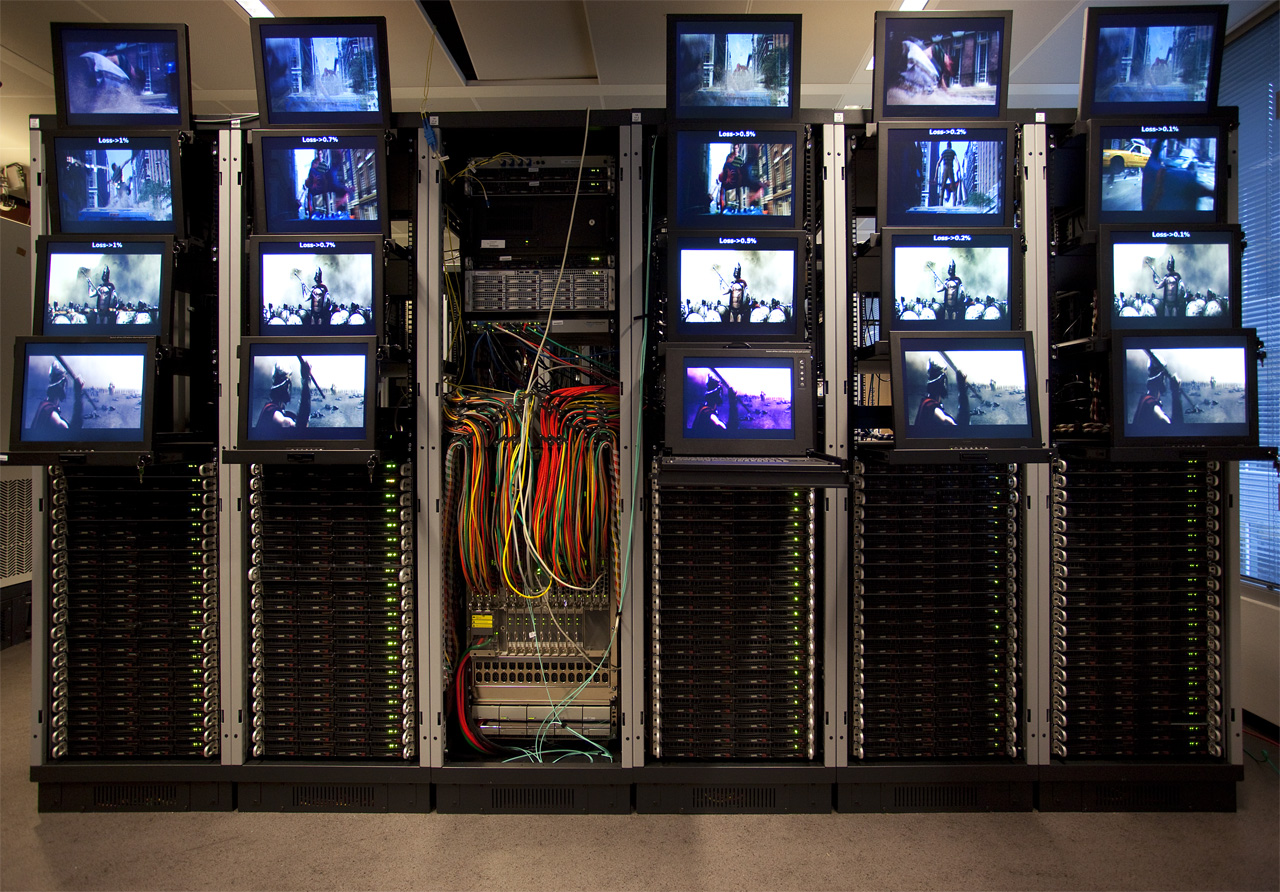
\includegraphics[scale=0.50]{figures/virtual-wall}
	\caption[De Virtual Wall bij iMinds]{De Virtual Wall bij iMinds\cite{virtual-wall-specs}}
	\label{fig-virtual-wall}
\end{figure}

\subsubsection{Overzicht opstelling}
\todo[inline]{Titel ok?}

De bedoeling van de opstelling op de \vwall{}  is om een situatie na te bootsen waarbij een groot aantal toestellen ondervraagd moet worden.
Omdat de \vwall{} gedeeld wordt door meerdere onderzoekers kunnen we natuurlijk niet zomaar de helft van de servers gebruiken voor ons experiment.
Bovendien hadden onze virtuele machines in VirtualBox genoeg met een core en 256 MB geheugen voor een \gls{snmp-agent}.
Dan zou een machine met twaalf cores en 24 GB geheugen natuurlijk zware \textit{overkill} zijn.
Wat we dus doen is een groot aantal virtuele machines opzetten op een paar van die servers.
Er zijn verschillende virtualisatietechnologieën die we kunnen aanwenden waaronder OpenVZ en Xen.
Vanwege problemen die verder besproken worden in \cref{probleem-virtualisatie-vwall}, werd er geopteerd voor \gls{lxc}.
Met \gls{lxc} kunnen we een 50-tal virtuele machines laten draaien op een enkele server.
We hebben dan uiteindelijk maar drie servers nodig: twee waarop de virtuele machines draaien en een waarop de \nwmretriever{} draait.
Elk van die 100 virtuele machines zal dan een eigen \gls{snmp-agent} draaien.

\subsubsection{Linux Containers}
\label{lxc}

\gls{lxc} is een lichte virtualisatietechnologie voor Linux die werkt op het niveau van het besturingssysteem.
Daarom gaat het niet om een volwaardige virtuele machine, maar voorziet het een virtuele omgeving met een eigen procesruimte, bestandssysteem en netwerkinterfaces.
\gls{lxc} maakt hiervoor gebruik van de resourcemanagement- en resource-isolatiefeatures in de kernel zoals \textit{\gls{cgroups}}\footnote{
	\gls{cgroups} zorgen voor de resource-isolatie van de CPU, het geheugen, I/O, netwerk enzovoort\cite{lxc-wiki}.
} en \textit{namespace isolation}\footnote{
	Namespace isolation zorgt ervoor dat applicaties een volledig geïsoleerd zicht hebben op het besturingssysteem,
	waaronder processen, het netwerk, gebruikers en bestandssystemen\cite{lxc-wiki}.
}\cite{lxc-explained, lxc-wiki}.


\subsubsection{Netwerkconfiguratie}

De fysieke netwerktopologie is zeer eenvoudig: de drie servers worden simpelweg met elkaar verbonden via een switch.
De Linux containers (vanaf nu nodes genoemd) zijn daarmee echter nog niet bereikbaar.
Daarvoor moet er op elk van de twee hostmachines een bridge\footnote{
	Ondanks het feit dat deze functie in Linux een bridge genoemd wordt, komt de functionaliteit ervan overeen met een switch.
	De naam komt van het feit dat ze een brug vormt tussen twee of meer netwerkverbindingen.
} geconfigureerd worden met enerzijds zijn eigen netwerkinterface
en anderzijds alle nodes die op die machine draaien.
Daarvoor moet je voor elke node twee virtuele interfaces aanmaken die met elkaar verbonden zijn.
Eén interface wijs je dan toe aan de bridge en de ander aan de node\cite{lxc-config}.
De commando's daarvoor zien er als volgt uit:

\begin{lstlisting}[caption={Linux containers verbinden met een bridge\cite{lxc-config}}]
# Bepaal de PID van de container vnode0:
$ pid=$(sudo lxc-info -pHn vnode0)

# Maak een paar virtuele interfaces aan die met elkaar verbonden zijn:
$ sudo ip link add name veth0 type veth peer name veth0_container

# Wijs een interface toe aan de bridge br0:
$ sudo brctl addif br0 veth0

# Wijs de andere interface toe aan de container:
$ sudo ip link set dev veth0_container netns $pid name veth0
\end{lstlisting}

Schematisch ziet de combinatie van de fysieke netwerkopstelling en de netwerkconfiguratie op de hosts er uit als in \cref{fig-vwall-opstelling}.

\begin{figure}[h]
	\centering
	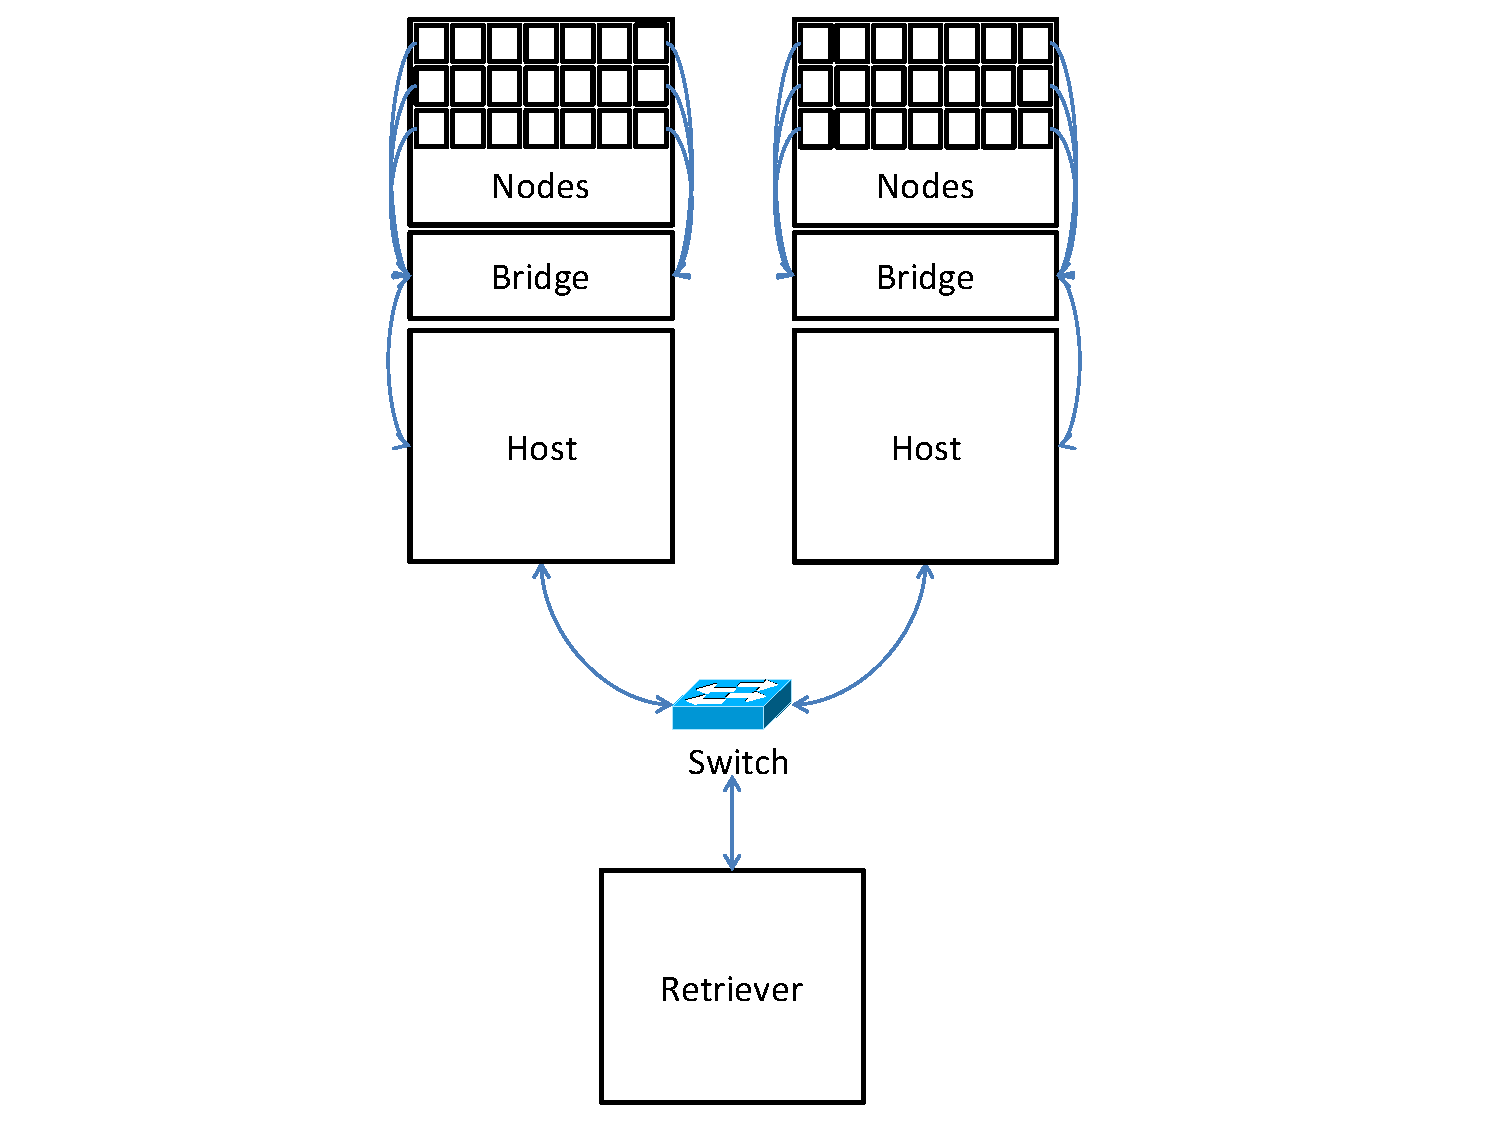
\includegraphics[scale=0.50]{figures/virtual-wall-opstelling}
	\caption{Netwerkopstelling \vwall{}}
	\label{fig-vwall-opstelling}
\end{figure}

\todo[inline]{Pijlen aanpassen in de figuur.}


\subsubsection{Softwareconfiguratie containers}

Alle 100 nodes hebben een gelijkaardige softwareconfiguratie als van onze virtuele machines in VirtualBox van \cref{virtualbox}.
De nodes zijn voorzien van hun eigen \gls{snmp-agent} en draaien het \gls{lldp}-protocol.
Het verschil met de kleinschalige opstelling is dat ze niet als bridge geconfigureerd zijn.
Het belangrijkste is dat elke node over voldoende gegevens beschikt die we kunnen opvragen,
en dat aantal kunnen we indien nodig makkelijk artificieel verhogen, door het creëren van VLAN's (zoals in \cref{rij-per-rij}).


\subsection{Impact databankinteracties}
\label{impact-db}

% In een voetnoot bij de profilertests in \cref{profiling} hebben we geschreven dat we over het hoofd hebben gezien dat we de databank op een SSD hadden geïnstalleerd.
% Daarbij hebben we de fout gemaakt door te vergelijken met resultaten

Als je de voetnoten gelezen hebt in onze tests met de profiler in \cref{profiling},
dan weet je dat we daar een fout hebben gemaakt door te vergelijken met resultaten waarbij we de databank geïnstalleerd hadden op een SSD.
Daardoor werd het probleem van het wegschrijven van de opgehaalde gegevens in de databank sterk geminimaliseerd.
Omdat de \nwmretriever{} en de databank in de \vwall{}opstelling geïnstalleerd werden op een traditionele harde schijf,
merkten we dan ook snel op dat we bijlange niet dezelfde performantiewinsten behaalden als bij onze kleinschalige tests.
Ook NetworkMining ondervond dezelfde performantieproblemen bij het wegschrijven naar de databank en hadden daarop een nieuwe versie ontwikkeld die als alternatief
de opgehaalde gegevens naar een XML-bestand kan wegschrijven.

Wegens tijdsgebrek hebben we het gebruik van bulk inserts niet meer kunnen implementeren.
Om toch de impact van het wegschrijven van de gegevens te kunnen meten,
hebben we een optie ingebouwd die deze databankinteracties simpelweg achterwege laat.

\subsubsection{Meetresultaten}

We doen de test met 1, 10 en 100 nodes en dat zowel voor de originele versie als de nieuwe versie die gebruik maakt van bulkrequests en log4net als loggingframework.
Om de tabelgrootte te beperken, vermelden we echter niet elke combinatie.
We doen opnieuw een SNMP walk van de mib-2- en enterprises-\glspl{oid}, nog steeds goed voor 3558 objecten.

\begin{table}[h]
\centering
\begin{tabular}{@{}ccrrrr@{}}
\toprule
\multicolumn{1}{l}{Nodes} & \multicolumn{1}{l}{Versie} & Insert & Uitvoeringstijd (s) & Factor & Factor nieuw vs oud \\ \midrule
\multirow{2}{*}{1}        & \multirow{2}{*}{Nieuw}     & Ja     & 6,634               &        &                     \\
                          &                            & Nee    & 2,669               & 2,49   &                     \\
\multirow{2}{*}{10}       & \multirow{2}{*}{Oud}       & Ja     & 77,333              &        &                     \\
                          &                            & Nee    & 29,762              & 2,60   &                     \\
\multirow{4}{*}{100}      & \multirow{2}{*}{Oud}       & Ja     & 1100,418            &        &                     \\
                          &                            & Nee    & 125,820             & 8,75   &                     \\
                          & \multirow{2}{*}{Nieuw}     & Ja     & 1051,373            &        & 1,05                \\
                          &                            & Nee    & 17,229              & 61,02  & 7,30                \\ \bottomrule
\end{tabular}
\caption{Impact van de databankinteracties}
\label{tabel-impact-db}
\end{table}

De resultaten zie je in \cref{tabel-impact-db}.
De eerste kolom duidt het aantal nodes aan, de tweede de versie, waarbij ''oud'' de originele versie aanduidt en ''nieuw'' de versie die gebruik maakt van bulkrequests en log4net.
De derde kolom geeft aan of de resultaten worden weggeschreven in de databank of niet, de vierde de gemiddelde uitvoeringstijd en de vijfde geeft aan hoeveel keer
sneller de versie zonder inserts is.
De laatste kolom tenslotte geeft aan hoeveel keer sneller de nieuwe versie is tegenover de oude versie, met en zonder inserts.

De resultaten laten een duidelijk beeld zien:
er is een gigantisch verschil in uitvoeringstijd indien men wel of niet de gegevens wegschrijft in de databank.
Gaande van 2,5 keer bij een tot tien nodes, tot ruim 60 keer sneller bij de nieuwe versie!
Het is duidelijk dat het aanpakken van de inserts een zeer hoge prioriteit moet krijgen en dat het gebruik van bulk inserts sterk aangeraden is.

We zien ook dat het verschil tussen de oude versie en de nieuwe versie verwaarloosbaar is bij een groot aantal nodes als men de databankinserts niet aanpakt:
de nieuwe versie is daar slechts 5\% sneller.
Maar als de retriever niet tegengehouden wordt door de databaseinserts, is de nieuwe versie ruim zeven keer sneller als er veel toestellen bevraagd moeten worden!
Het is dus belangrijk om de databankinteracties aan te pakken om de nieuwe versie van de \nwmretriever{} volledig tot zijn recht te laten komen.
\todo[inline]{Bij de kleinschalige tests zagen we al dat de nieuwe versie bij slechts een toestel al vier keer sneller was.
De snelheidswinst neemt dus sterk toe naarmate het aantal toestellen toeneemt dat bevraagd moet worden.}

\subsubsection{Conclusie}

Zowel bij kleine, maar vooral bij grote aantallen toestellen die bevraagd moet worden is er een grote impact op de uitvoeringstijd door de databankinteracties.
Het gebruik van bulk inserts moet dan ook een topprioriteit gemaakt worden.
Een mogelijke manier van werken zou zijn om het wegschrijven van gegevens in een aparte thread te laten verlopen.
Zo zijn er geen 50 threads die tegelijkertijd proberen hun data weg te schrijven naar de databank.
Men kan een tabel in het geheugen bijhouden om initieel de resultaten in bij te houden.
In een aparte thread kan men dan de data uit die tabel wegschrijven naar de databank in zo groot mogelijke blokken met bulk inserts.

Omdat het implementeren en testen van die functionaliteit redelijk wat tijd in beslag kan nemen,
kan men overwegen om op korte termijn de databank op te slaan op een SSD om zo het effect van de databankinteracties te minimaliseren.


\subsection{Benchmarks uitvoeringstijd}
\label{uitvoeringstijd-vwall}

Om de schaalbaarheid van de \nwmretriever{} te verbeteren hebben we al twee grote aanpassingen gedaan aan de \nwmretriever{},
namelijk het gebruik van bulkrequests en een alternatief loggingframework.
In deze paragraaf beoordelen we de uitvoeringstijd van de nieuwe versie van de \nwmretriever{} met onze aanpassingen ten opzichte van de oude.
In \cref{impact-db} hebben we ook gezien dat de databankinteracties een grote negatieve impact hebben op de uitvoeringstijd.
Omdat we daarvoor geen oplossing hebben geïmplementeerd, moeten we het stellen bij het vergelijken van de uitvoeringstijd met en zonder databankinteracties.
Ten slotte bekijken we ook de invloed van het aantal te bevragen toestellen op de uitvoeringstijd en op basis daarvan
doen we een schatting voor het opvragen van tot 10.000 toestellen.{\todo{Verduidelijk.}}

\subsubsection{Uitvoeringstijd op grote schaal}

De uitvoeringstijd van de \nwmretriever{} op grote schaal hebben we al gemeten in de paragraaf over de impact van de databankinteracties.
We nemen die resultaten er bijgevolg weer bij.
In die paragraaf hebben we al gezien dat het verschil tussen de oude versie en de nieuwe slechts 5\% bedraagt
als de gegevens in de databank weggeschreven moeten worden.
Wanneer dat niet het geval is, is de nieuwe versie ruim zever keer sneller dan de oude!
Het is dus van absoluut belang dat dit probleem aangepakt wordt, of dat er gebruik gemaakt wordt van een SSD om de databank op te slaan.
Natuurlijk zal een alternatieve implementatie met bulk inserts niet exact 7,3 keer sneller zijn, maar het geeft wel een goed idee
van hoeveel sneller de \nwmretriever{} zou kunnen gaan.

\begin{table}[h]
\centering
\begin{tabular}{@{}ccrrr@{}}
\toprule
\multicolumn{1}{l}{Nodes} & \multicolumn{1}{l}{Versie} & Insert & Uitvoeringstijd (s) & Factor nieuw vs oud \\ \midrule
\multirow{4}{*}{100}      & \multirow{2}{*}{Oud}       & Ja     & 1100,418            &                     \\
                          &                            & Nee    & 125,820             &                     \\
                          & \multirow{2}{*}{Nieuw}     & Ja     & 1051,373            & 1,05                \\
                          &                            & Nee    & 17,229              & 7,30                \\ \bottomrule
\end{tabular}
\caption{Uitvoeringstijd van de \nwmretriever{} op grote schaal}
\label{tabel-uitvoeringstijd-vwall}
\end{table}

\subsubsection{Invloed aantal bevraagde toestellen}

In \cref{tabel-uitvoeringstijd-aantalnodes} zien we de gemiddelde uitvoeringstijd van de \nwmretriever{} bij 1, 10, 50 en 100 nodes, zonder databankinteracties.
Alhoewel er tot 50 toestellen tegelijkertijd opgevraagd kunnen worden, zien we toch dat de uitvoeringstijd ook bij minder dan 50 toestellen toeneemt.

\begin{table}[h]
\centering
\begin{tabular}{@{}lrrrr@{}}
\toprule
                    & 1 node & 10 nodes & 50 nodes & 100 nodes \\ \midrule
Uitvoeringstijd (s) & 2,669  & 4,013    & 8,590    & 17,351    \\ \bottomrule
\end{tabular}
\caption{Uitvoeringstijd bij een verschillend aantal toestellen}
\label{tabel-uitvoeringstijd-aantalnodes}
\end{table}

Om te zien hoe sterk de uitvoeringstijd juist toeneemt met het aantal te bevragen toestellen,
hebben we de resultaten in een grafiek voorgesteld en de trendlijn getekend.

Het is duidelijk dat er een lineair verband is tussen het aantal toestellen dat moet bevraagd worden en de uitvoeringstijd.
De trendlijn leert ons dat elk \textit{extra} toestel dat bevraagd moet worden ongeveer 0,15 seconden extra vraagt.

\begin{figure}[h]
	\centering
	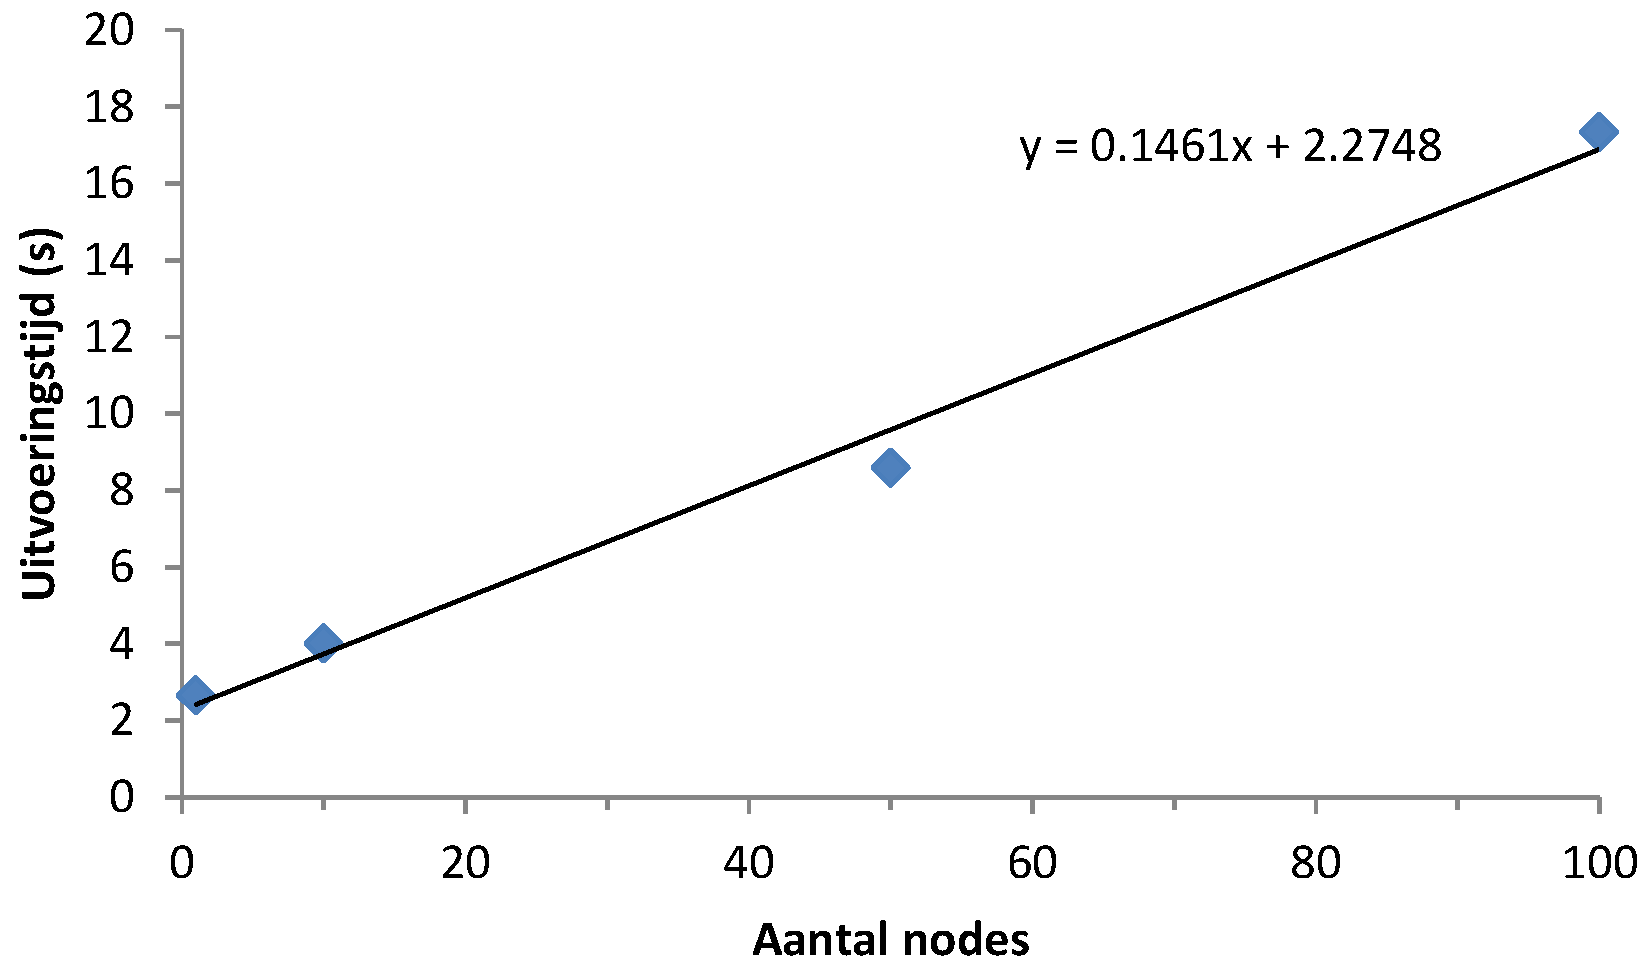
\includegraphics[scale=0.40]{figures/uitvoeringstijd}
	\caption{Uitvoeringstijd bij een verschillend aantal toestellen}
	\label{fig-uitvoeringstijd}
\end{figure}

In \cref{tabel-theoretische-uitvoeringstijd} hebben we de theoretische uitvoeringstijd berekend aan de hand van de bovenstaande formule voor 1 tot 10.000 toestellen.
We zien dat de resultaten weinig afwijken van de reële resultaten.
De theoretische uitvoeringstijd voor 1000 toestellen bedraagt amper 2,5 minuten en voor 10.000 toestellen gaat het om minder dan 25 minuten.

\begin{table}[h]
\centering
\begin{tabular}{@{}rr@{}}
\toprule
Toestellen & Uitvoeringstijd (s) \\ \midrule
1          & 2,669               \\
2          & 2,815               \\
3          & 2,961               \\
4          & 3,107               \\
5          & 3,253               \\
10         & 3,984               \\
20         & 5,445               \\
30         & 6,906               \\
40         & 8,367               \\
50         & 9,828               \\
100        & 17,133              \\
1000       & 148,623             \\
10000      & 1463,523            \\ \bottomrule
\end{tabular}
\caption{Theoretische uitvoeringstijd bij een verschillend aantal toestellen}
\label{tabel-theoretische-uitvoeringstijd}
\end{table}

\subsubsection{Conclusie}

Op voorwaarde dat het probleem met de databankinteracties aangepakt wordt, kunnen we besluiten dat de gemaakte verbeteringen
al een zeer positieve invloed hebben op de uitvoeringstijd van de \nwmretriever{} op grote schaal.

Ook de impact van het aantal te bevragen toestellen op de uitvoeringstijd blijft zeer beperkt met ongeveer 0,15 seconden extra per bijkomend toestel.

Een lage uitvoeringstijd is echter niet het enige criterium om te beslissen of de retriever goed schaalbaar is:
ook met andere resources moet goed omgegaan worden, zoals CPU, geheugen en bandbreedte.
Die zaken onderzoeken we in de volgende paragrafen.


\subsection{Benchmarks CPU-gebruik}
\label{cpu-gebruik}

In deze paragraaf bekijken we de invloed van het aantal op te vragen toestellen op het CPU-gebruik van de \nwmretriever{}.
We bekijken ook het CPU-gebruik gedurende de uitvoering van het programma en bespreken het gedrag ervan.
Ook het aantal threads gedurende de uitvoering die gebruikt worden om de toestellen te bevragen nemen we onder de loep.

\subsubsection{Meetresultaten}

In \cref{fig-cpu-aantalnodes} zien we het CPU-gebruik van de \nwmretriever{} bij een verschillend aantal nodes.
Misschien vraag je je af waarom het CPU-gebruik over de 100\% gaat.
De reden daarvoor is omdat de server waarop de retriever draait in totaal 16 cores heeft.
De belasting van een volledige core komt dan overeen met 100\%, twee cores met 200\% enzovoort.
Als je dus een CPU-gebruik van 900\% ziet, dan komt dat ongeveer overeen met een volledige belasting van 9 cores.
In de praktijk wordt de werklast echter verdeeld over meer dan 9 cores zodat ze niet allemaal volledig belast worden.

We zien dat het CPU-gebruik meestijgt met het aantal nodes.
Vanaf 50 nodes echter stijgt het CPU-gebruik niet verder voorbij iets meer dan 900\%.
Dat is logisch, want er worden maar maximaal 50 toestellen tegelijkertijd opgevraagd.

Naar het einde toe zien we iets vreemds.
We verwachten dat, eenmaal het resterend aantal te bevragen toestellen onder de 50 zakt,
het CPU-gebruik geleidelijk aan zou moeten zakken tot 0\% wanneer alle toestellen bevraagd zijn en het programma afsluit.
Wat we echter zien is dat het CPU-gebruik bij 100 nodes vanaf 13 seconden sterk zakt om kort daarna weer sterk te stijgen.

Met behulp van het logbestand en Wireshark kunnen we de oorzaak vinden.
Met het logbestand kunnen we zien hoeveel threads er actief zijn om toestellen te bevragen,
en met Wireshark kunnen we zien hoeveel requests onderweg zijn.
Een grafiek van het aantal retrieverthreads zie je in \cref{fig-retrieverthreads}.

Het probleem dat zich voordoet is het volgende:
er zijn op het einde minder dan 50 toestellen die nog moeten bevraagd worden, waardoor er minder dan 50 threads actief zijn.
In de grafiek met het aantal threads zie je rond 13 seconden dat het aantal threads daalt,
omdat de laatste antwoorden binnenkomen van een aantal toestellen die dus afgewerkt zijn.
Omdat er verder geen toestellen meer zijn worden er ook geen nieuwe threads meer gestart.
De threads die wel nog actief zijn blijken uit Wireshark allemaal nog te wachten op een antwoord van de toestellen en hebben dus tijdelijk niks te doen.
Wanneer de antwoorden kort daarna aankomen, krijg je opnieuw een piek in het CPU-gebruik door de gegevens die moeten verwerkt worden.
Tegelijkertijd zie je dat het aantal threads verder afneemt naarmate de laatste toestellen afgewerkt worden.

\begin{figure}[h]
	\centering
	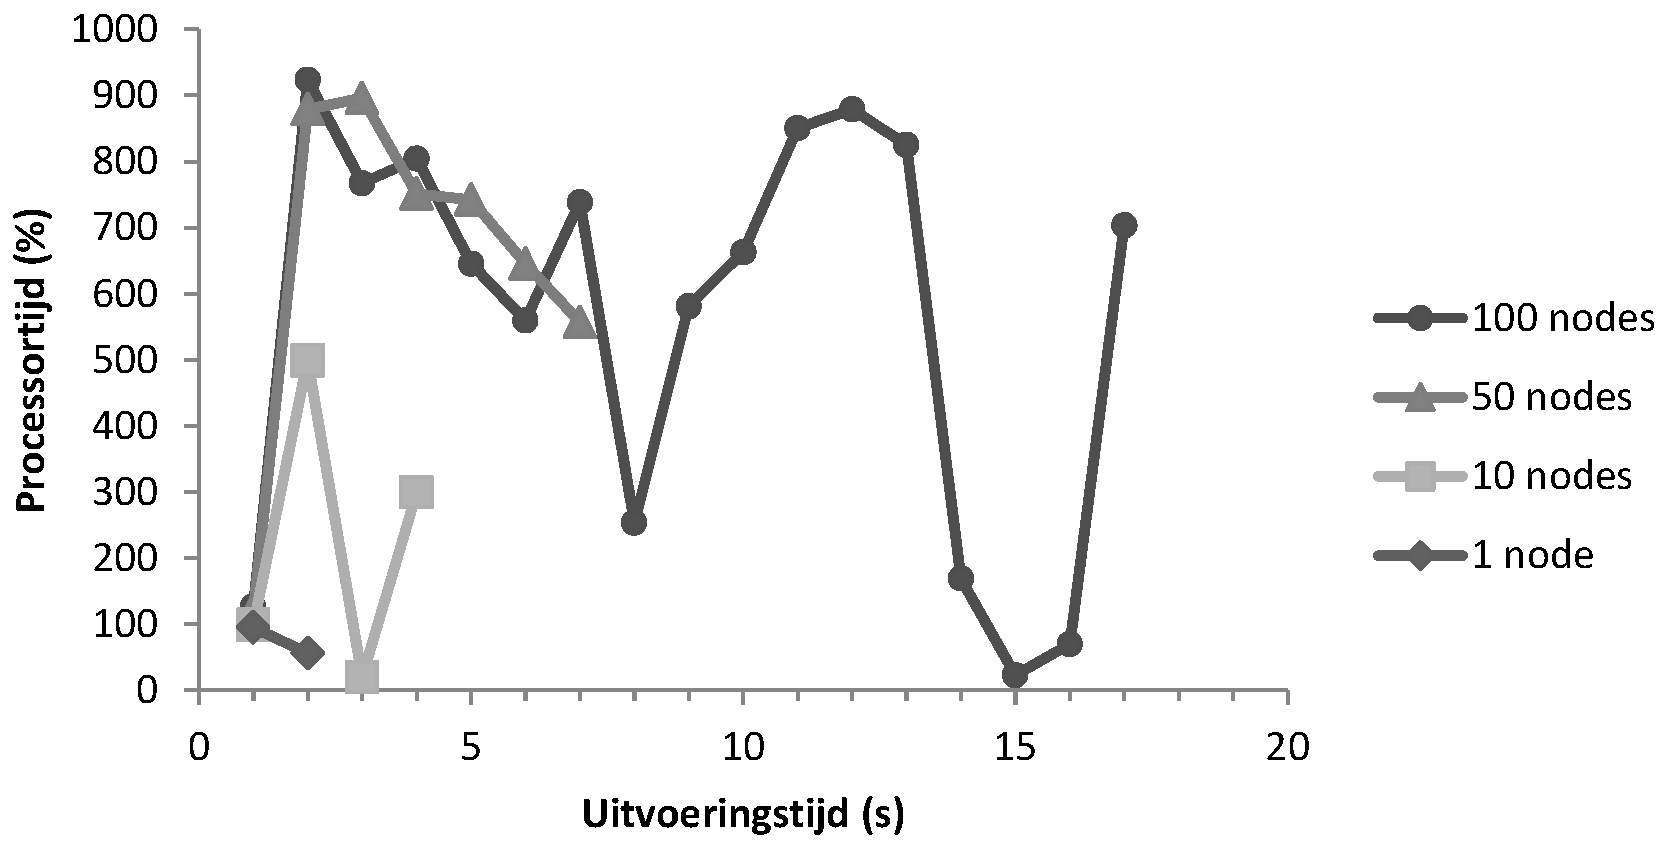
\includegraphics[scale=0.40]{figures/cpu-100nodes}
	\caption{CPU-gebruik bij verschillend aantal nodes}
	\label{fig-cpu-aantalnodes}
\end{figure}

\begin{figure}[h]
	\centering
	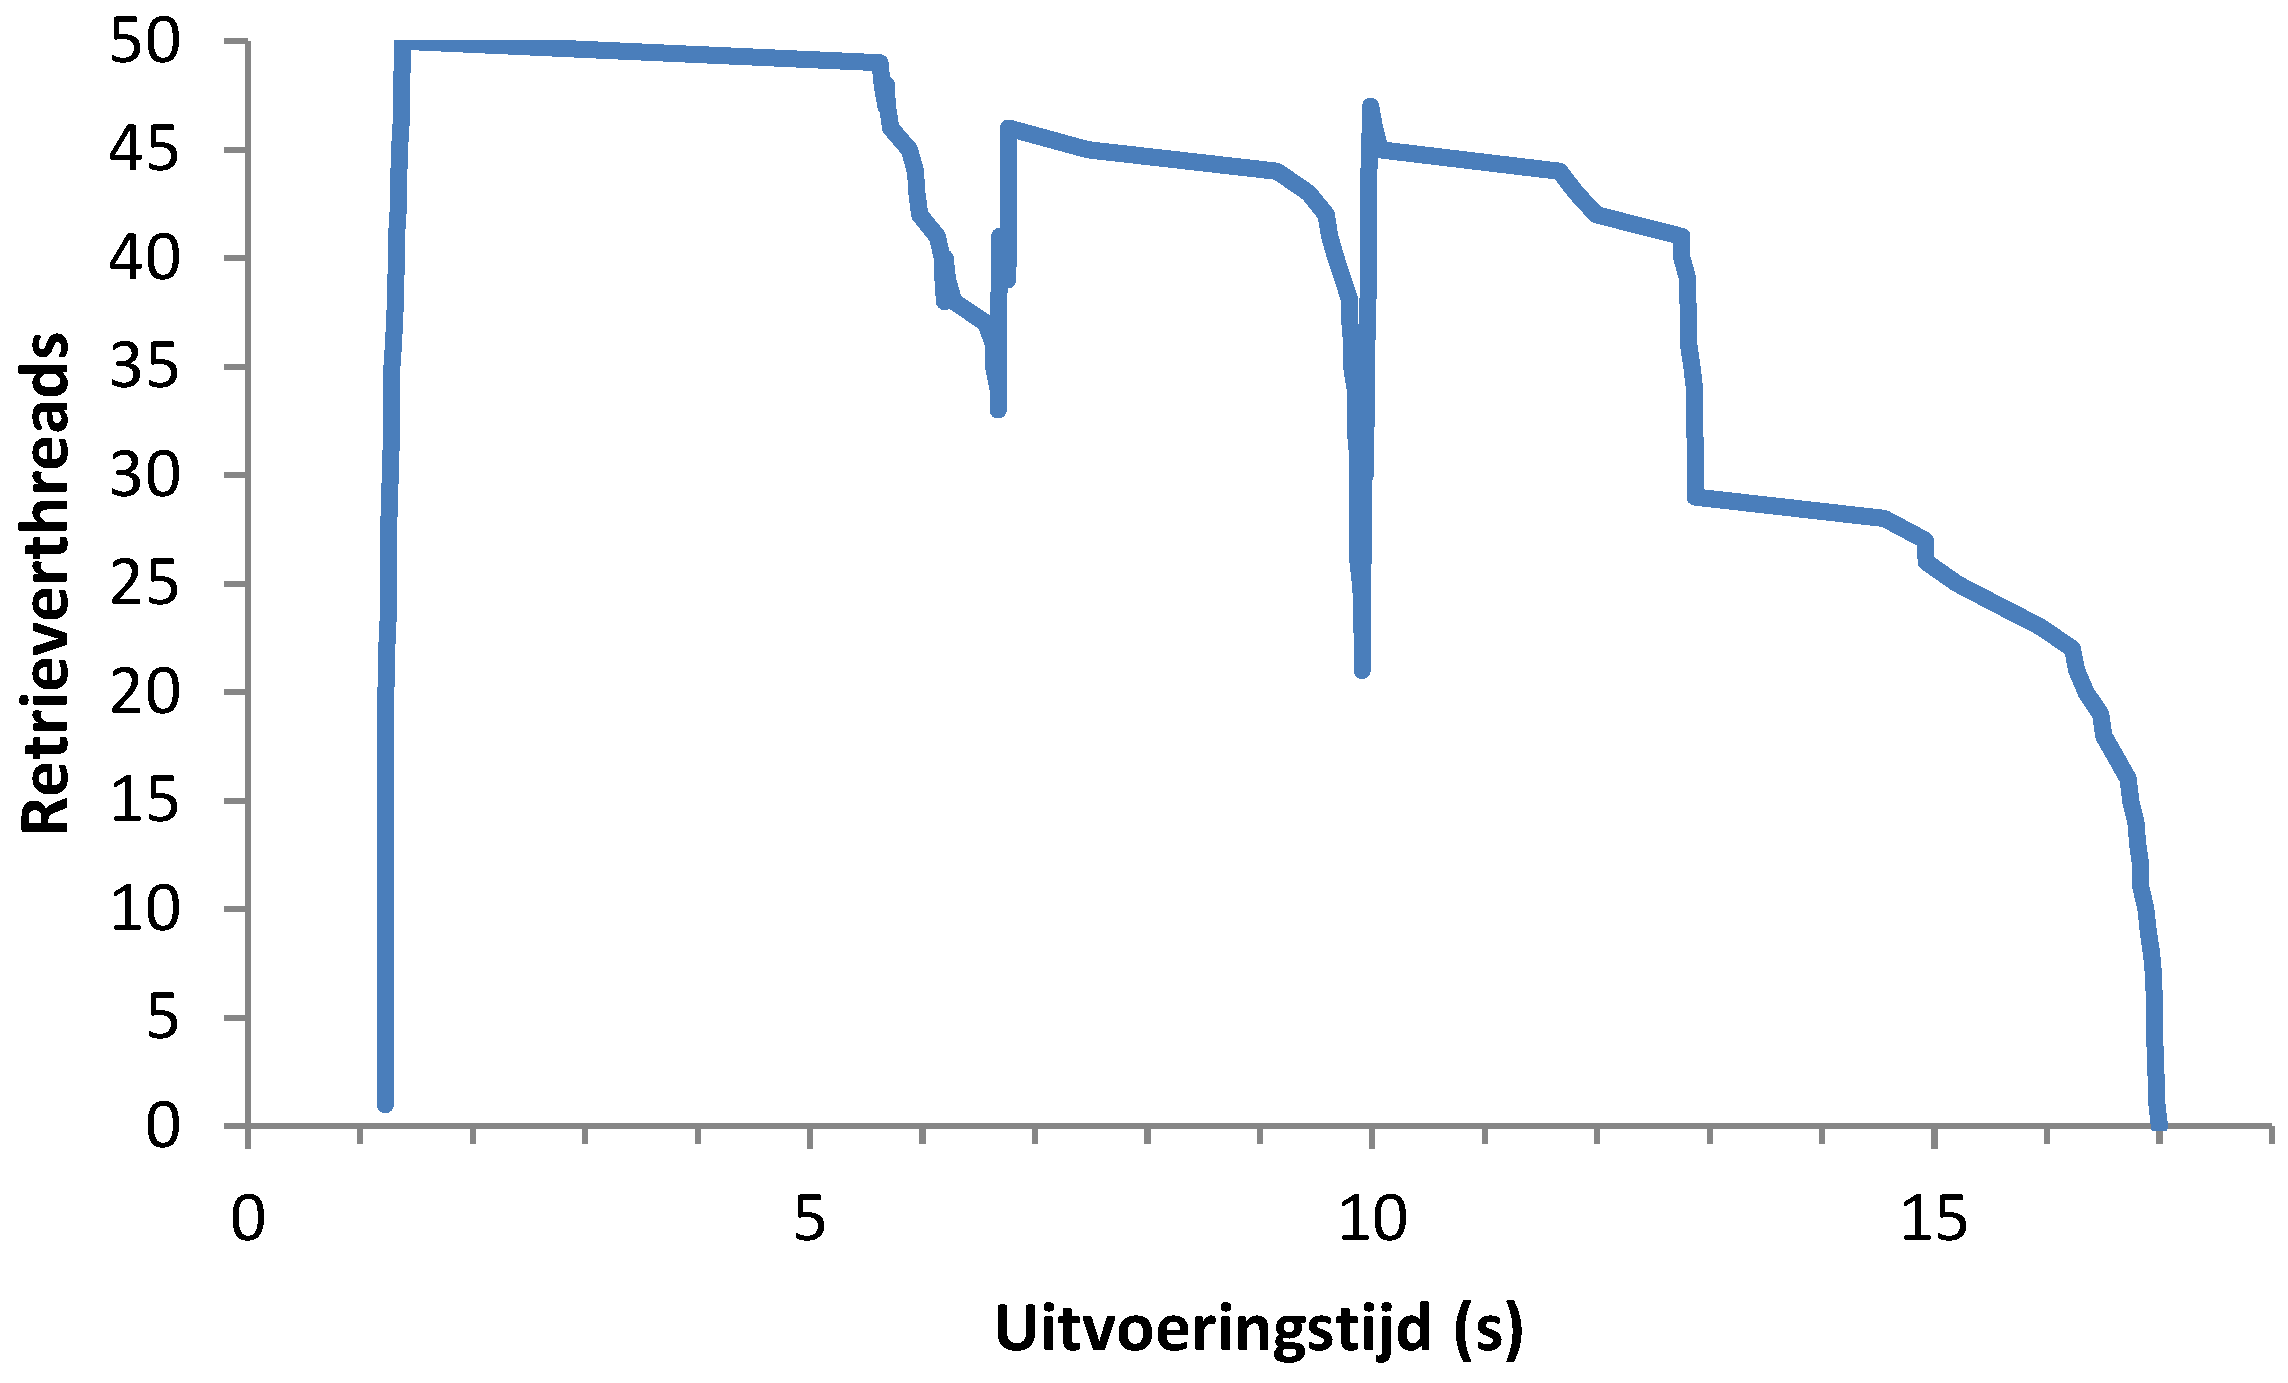
\includegraphics[scale=0.30]{figures/threads-100nodes}
	\caption{Aantal retrieverthreads tijdens de uitvoer van de \nwmretriever{}}
	\label{fig-retrieverthreads}
\end{figure}

% Put this paragraph in a minipage so it doesn't get split up across a pagebreak.
\begin{minipage}{\textwidth}
In de grafiek met het aantal retrieverthreads zien we trouwens ook een probleem met hoe de threads beheerd worden.
Zoals uitgelegd in \cref{werking} worden in de oude versie die wij gebruiken de threads in een lijst bijgehouden,
en wordt er gewacht op de eerste thread om te voltooien eer er nieuwe threads gestart worden.
Het probleem daarbij is dat het niet noodzakelijk de eerst gestarte thread is die eerst klaar zal zijn.
Terwijl er gewacht wordt op de eerste thread kunnen er gerust al andere threads klaar zijn en dat zien we ook in de grafiek rond 5 en 10 seconden.
Het aantal threads daalt, maar doordat er gewacht wordt op de eerste thread, duurt het even eer er nieuwe threads aangemaakt worden.
Dit probleem werd doorgegeven aan NetworkMining en werd vrij snel opgelost in een nieuwe versie.
\end{minipage}

\subsubsection{Conclusie}

Doordat er maximaal 50 toestellen tegelijkertijd bevraagd worden blijft het CPU-gebruik ook constant bij het bevragen van meer 50 toestellen.
Door het constant houden van het aantal threads zien we echter dat niet alle rekenkracht benut wordt.
Alhoewel er 16 cores beschikbaar zijn, er is maar een CPU-belasting die overeenkomt met een volledige belasting van iets meer dan 9 cores.

Het beheren van threads zou dus beter aangepakt kunnen worden:
enerzijds bij het bepalen van het aantal threads dat moet gebruikt worden, afhankelijk van hoeveel rekenkracht er nog over is
(en het RAM- en bandbreedtegebruik, maar die spelen een veel kleinere rol zoals we verder zullen zien).
Anderzijds moeten ook nieuwe threads gestart worden van zodra een toestel afgewerkt is,
maar dat is een probleem dat reeds opgelost werd door NetworkMining.

\subsection{Benchmarks geheugenverbruik}
\label{benchmarks-geheugengebruik}

Over het geheugenverbruik valt er weinig te vertellen.
We bekijken opnieuw de invloed van het aantal te bevragen toestellen op het geheugengebruik maar
we zullen zien dat de conclusies die we gemaakt hebben in de vorige paragraaf hier ook van toepassing zijn.

\subsubsection{Meetresultaten}

In \cref{fig-ram-aantalnodes} zien we het geheugengebruik van de \nwmretriever{} bij een verschillend aantal nodes.
Net als bij het CPU-gebruik zien we dat het geheugenverbruik meestijgt met het aantal op te vragen toestellen.
En ook hier stijgt het geheugengebruik niet verder als er meer dan 50 toestellen moeten bevraagd worden.

Het geheugenverbruik blijft relatief constant gedurende de uitvoer van het programma.
Er is een initiële piek wanneer de threads aangemaakt worden en het verbruik zakt pas wanneer het aantal threads daalt.
De hoeveelheid geheugen dat gebruikt wordt valt op zich ook zeer goed mee: bij 50 of meer toestellen is er een piekverbruik van ongeveer 80 MB.

\begin{figure}[h]
	\centering
	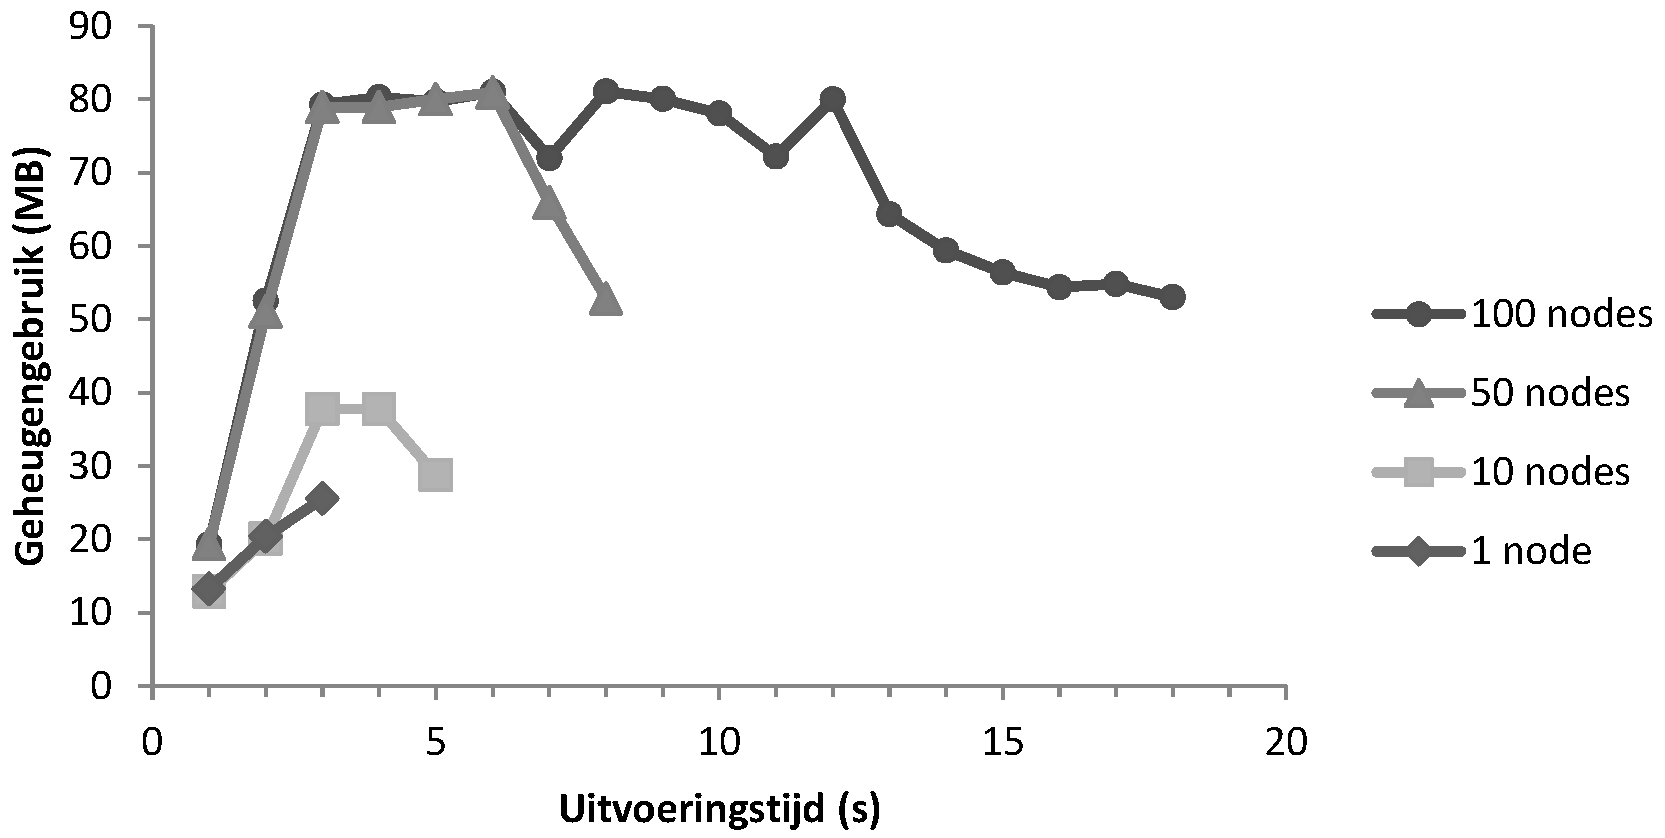
\includegraphics[scale=0.40]{figures/ram-100nodes}
	\caption{Geheugenverbruik bij verschillend aantal nodes}
	\label{fig-ram-aantalnodes}
\end{figure}

\subsubsection{Conclusie}

Net als het CPU-gebruik stijgt het geheugengebruik niet verder als er meer dan 50 toestellen bevraagd worden.
Het geheugengebruik is gedurende de uitvoer vrij constant en met een maximaal verbruik van ongeveer 80 MB kunnen we zeggen dat
de \nwmretriever{} absoluut niet veel geheugen nodig heeft.

Mocht het voorstel om de impact van de databankinteracties te beperken, geïmplementeerd worden (\cref{impact-db}),
is er duidelijk nog genoeg geheugen vrij om een tabel in het geheugen te houden alvorens ze in de databank weg te schrijven. 


\subsection{Benchmarks bandbreedte}
\label{benchmarks-bandbreedte}

In deze paragraaf bekijken we het bandbreedteverbruik van de \nwmretriever{}.
We vergelijken het bandbreedteverbruik van een SNMP walk op basis van GETNEXT- en GETBULK-requests.
Ook gaan we na wat de invloed is van het aantal te bevragen toestellen op het bandbreedtegebruik.

\subsubsection{SNMP Walk met GETNEXT- versus GETBULK-requests}

In \cref{tabel-bandbreedte-walk-vs-bulk} staan de netwerkstatistieken voor een SNMP walk op basis van GETNEXT- en GETBULK-requests.
Weinig verrassend is dat er met bulkrequests een stuk minder pakketten verstuurd worden dan ontvangen.
Vermits we 50 objecten per request opvragen, zijn er ook ongeveer 50 keer minder pakketten die moeten verstuurd worden.
Omdat er veel minder pakketten worden verstuurd en ontvangen, worden er natuurlijk ook minder bytes verstuurd en ontvangen.
Minder pakketten wil ook zeggen minder overhead door de headers van de pakketten.
En omdat er in totaal minder data is verstuurd en ontvangen, was er ook gemiddeld minder bandbreedte nodig.


\begin{table}[h]
\centering
\begin{tabular}{@{}lrr@{}}
\toprule
                           & Walk   & Bulkwalk \\ \midrule
Pakketten verstuurd        & 2752   & 56       \\
Pakketten ontvangen        & 2752   & 56       \\
KiloBytes verstuurd        & 234,86 & 4,78     \\
KiloBytes ontvangen        & 239,83 & 54,25    \\
Gem. KiloBytes per seconde & 79,82  & 40,23    \\
Gem. Megabits per seconde  & 0,65   & 0,33     \\ \bottomrule
\end{tabular}
\caption{Netwerkstatistieken SNMP walk met GETNEXT- versus GETBULK-requests}
\label{tabel-bandbreedte-walk-vs-bulk}
\end{table}

We zien dit ook terug in \cref{fig-bandbreedte-walk,fig-bandbreedte-bulkwalk} die de bandbreedte tonen gedurende
de SNMP walk met respectievelijk GETNEXT- en GETBULK-requests.
De fluctuatie die je ziet in beide grafieken is trouwens enkel te wijten aan de fluctuatie in responstijd van de \gls{snmp-agent}.
De verwerkingstijd aan de kant van de retriever, of de tijd die nodig is om een nieuwe request te versturen, is daarentegen zeer consistent.
De resultaten werden hierbij echter niet weggeschreven in de databank.

\begin{figure}[h]
	\centering
	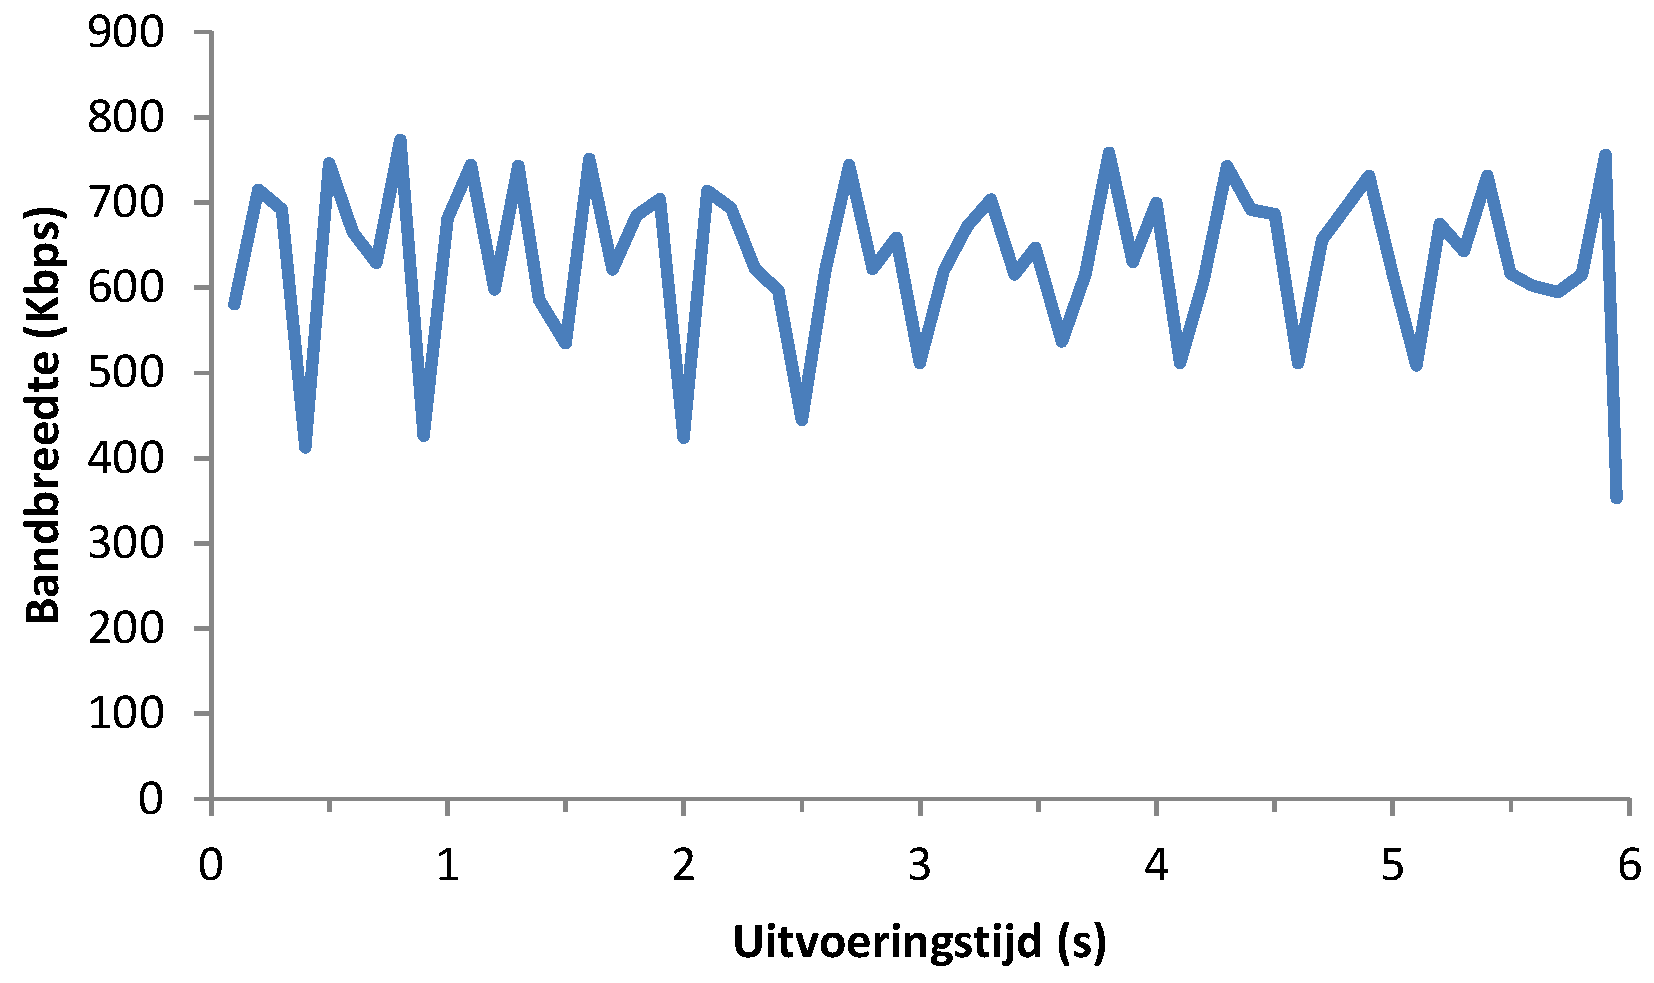
\includegraphics[scale=0.40]{figures/bandbreedte/snmpwalk}
	\caption{Bandbreedte SNMP walk met GETNEXT-requests}
	\label{fig-bandbreedte-walk}
\end{figure}

\begin{figure}[h]
	\centering
	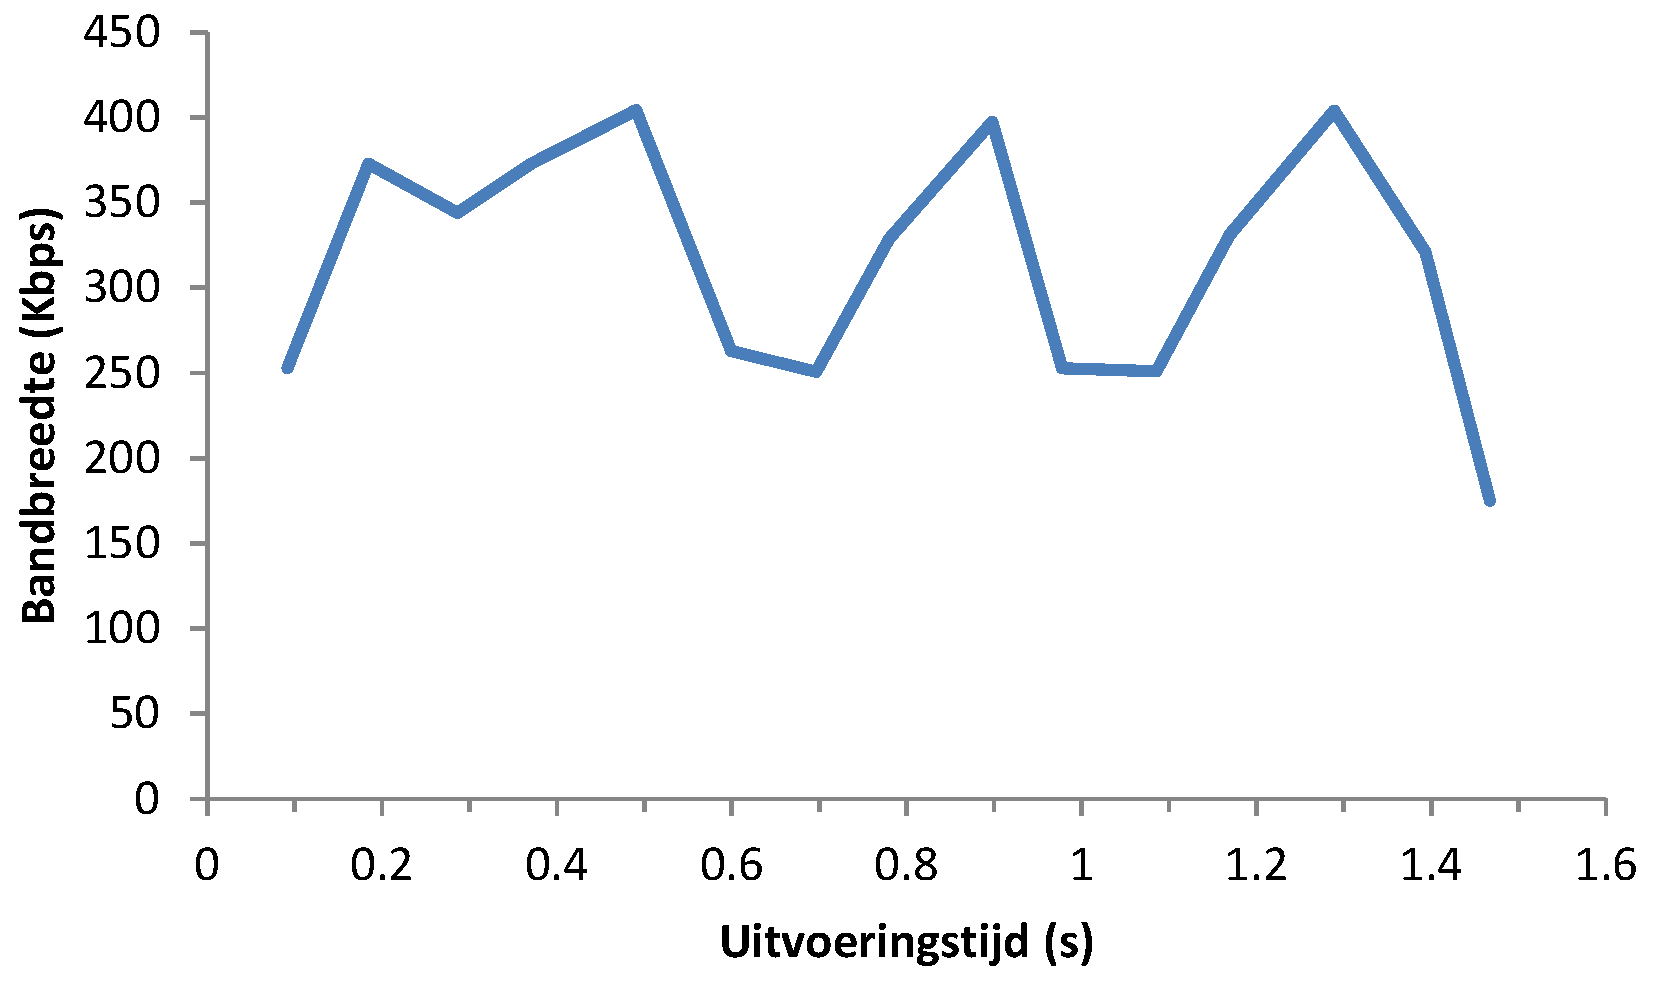
\includegraphics[scale=0.40]{figures/bandbreedte/snmpbulkwalk}
	\caption{Bandbreedte SNMP walk met GETBULK-requests}
	\label{fig-bandbreedte-bulkwalk}
\end{figure}


\subsubsection{Invloed aantal ondervraagde nodes}

In \cref{tabel-bandbreedte-aantalnodes} zien we de netwerkstatistieken voor 1, 10, 50 en 100 nodes.
Omdat de toestellen quasi gelijk zijn aan elkaar, zien we dat het aantal pakketten en de hoeveelheid data lineair stijgt met het aantal nodes.
Bij het gemiddelde bandbreedteverbruik is dat echter niet het geval doordat meer nodes opvragen langer duurt.
Ondanks het feit dat de toestellen tegelijkertijd opgevraagd worden, duurt het toch iets langer om meerdere toestellen op te vragen.
Laat ons als voorbeeld het verschil tussen een en tien nodes nemen.
Er zijn wel tien keer meer toestellen op te vragen, maar er wordt bijna twee keer langer over gedaan.
Daardoor stijgt het bandbreedteverbruik dus ongeveer maar met een factor vijf in plaats van met een factor tien.

\begin{table}[h]
\centering
\begin{tabular}{@{}lrrrr@{}}
\toprule
                           & 1 node & 10 nodes & 50 nodes & 100 nodes \\ \midrule
Pakketten verstuurd        & 72     & 648      & 3507     & 7093      \\
Pakketten ontvangen        & 72     & 648      & 3507     & 7093      \\
KiloBytes verstuurd        & 6,75   & 60,75    & 328,10   & 663,70    \\
KiloBytes ontvangen        & 97,82  & 880,44   & 4.762,68  & 9.633,34   \\
Gem. KiloBytes per seconde & 84,64  & 398,51   & 730,84   & 655,82    \\
Gem. Megabits per seconde  & 0,69   & 3,27     & 5,99     & 5,37      \\
Tijd\textsuperscript{*} (s)& 1,235  & 2,362    & 6,966    & 15,701    \\ \midrule[.5pt]
\multicolumn{4}{l}{\textsuperscript{*} \footnotesize{Benodigde tijd enkel voor het SNMP-verkeer}}
\end{tabular}
\caption{Netwerkstatistieken voor een verschillend aantal nodes}
\label{tabel-bandbreedte-aantalnodes}
\end{table}

% Put this paragraph in a minipage so it doesn't get split up across a pagebreak, between the graph and the table.
\begin{minipage}{\textwidth}
Het bandbreedteverbruik zou ook niet verder mogen stijgen als er meer dan 50 toestellen bevraagd worden.
We zien zelfs dat ze daalt.
Als we naar de grafiek van het bandbreedteverbruik bij 100 nodes kijken in \cref{fig-bandbreedte-100-nodes}
zien we snel waarom.
Ook in het bandbreedteverbruik zien we hetzelfde fenomeen terug als bij het CPU-gebruik in \cref{cpu-gebruik}:
een dip gevolgd door een piek in het verbruik naar het einde toe.
Als er gelijktijdig gewacht wordt op antwoorden van de toestellen zal het bandbreedteverbruik op dat moment natuurlijk ook zakken.
\end{minipage}

\begin{figure}[h]
	\centering
	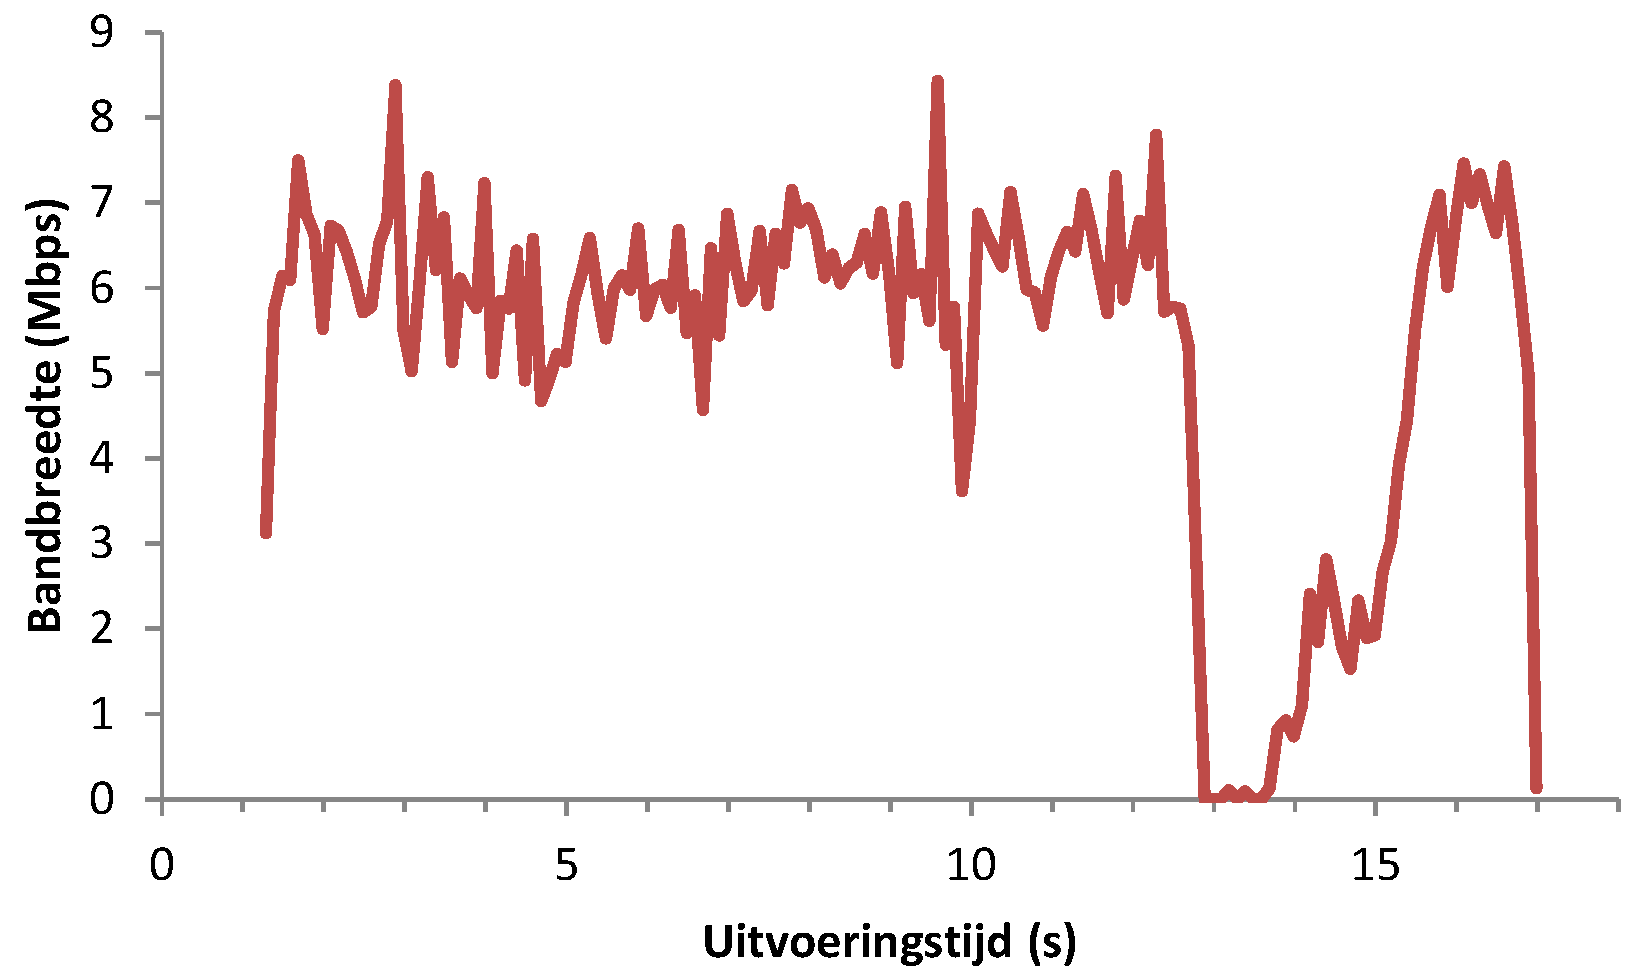
\includegraphics[scale=0.40]{figures/bandbreedte/bandbreedte-100nodes}
	\caption{Bandbreedte bij bevragen 100 nodes}
	\label{fig-bandbreedte-100-nodes}
\end{figure}

Vandaar dus dat het gemiddelde bandbreedteverbruik lager uitvalt.
De mediaan van het bandbreedteverbruik valt bij 100 nodes op bijna 6 Mbps, wat wel overeenkomt met het verbruik van 50 nodes.

Het bandbreedteverbruik valt op zich ook zeer goed mee, als je rekening houdt met het feit dat netwerkverbindingen meestal 100 Mbps of zelfs al 1 Gbps zijn.
In geval van een verbinding van 100 Mbps gaat het om een belasting van 6\%, bij een verbinding van 1 Gbps zelfs maar om een belasting van 0,6\%.

\subsubsection{Conclusie}

Naast de uitvoeringstijd is er nog een voordeel bij het gebruik van bulkrequests:
zowel het totale dataverkeer als de benodigde bandbreedte vallen een stuk lager uit dan bij GETNEXT-requests.

Net als bij het CPU- en geheugengebruik kunnen we opnieuw vaststellen dat het bandbreedteverbruik niet verder stijgt als er meer dan 50 toestellen bevraagd worden.
Ook over het bandbreedteverbruik hoeven we ons dus weinig zorgen te maken.
De bevragingen kunnen zelfs 's nachts ingepland worden, zodat er helemaal geen impact is op het netwerkverkeer tijdens de werkuren.